%%%%%%%%%%%%%%%%%%%%%%%%%%%%%%%%%%%%%%%%%%%%%%%%%%%%%%%%%%%%%%%%%%%%
%%%%%%%%%%%%%%%%%%%%%%%%%%%%%%%%%%%%%%%%%%%%%%%%%%%%%%%%%%%%%%%%%%%%
\section{Introduction}
\label{sec:Intro}

The last several decades have seen an increasing reliance upon quantitative predictions from computational, simulation-based models of physical systems to inform engineering design, predict the behavior of physical systems, and even shape public policy, e.g., see [TK - need citation] for just a few such examples.
It is therefore more important than ever to quantify, and reduce whenever possible, the uncertainties impacting such models.
Unfortunately, many key characteristics governing system behavior, described as model inputs (referred to here as parameters), are often hidden from direct observation.
When observable model output data are sensitive to variations in these parameters, we formulate and solve inverse problems using this output data to quantify uncertainties in parameters.
Inverse problems therefore play a vital role in the uncertainty quantification (UQ) community.

In UQ, uncertainties are categorized as being either aleatoric (i.e., irreducible) or epistemic (i.e., reducible) in nature, which are often quantitatively described and interpreted in distinct ways.
Below, we use abstractions of conceptual examples to distinguish how both types of uncertainties arise in parameters and impact the type of inverse problem that is solved to quantify these uncertainties.
% and their associated inverse problems while simultaneously comparing and contrasting methodologies for solving these problems.
This further serves to highlight the contributions of this work.

Consider modeling the manufacturing process of an engineered system involving various electrical or mechanical components.
The intrinsic variability in component properties, e.g., due to impurities in raw materials used in their construction, are aleatoric in nature.
%These are quantitatively characterized as probability measures.
Component properties define a sample space (the set of all possible outcomes), and combining this sample space with a description of measurable events along with a probability measure defines a probability space.
Scalar-valued model parameters associated with component properties defines a random vector (i.e., a measurable function) from this probability space of components into the parameters required by the model.
Subsequently, the mapping from parameters to observable model outputs defines what we refer to as a Quantities of Interest (QoI) map.
Observation of a probability measure on the range of the QoI map leads to the formulation of a stochastic inverse problem (SIP) where the goal is to pullback the observed probability measure onto the space of parameters.
Conceptually, a pullback measure is observation-consistent in the sense that its push-forward through the QoI map matches the observed probability measure.

While it is possible to construct explicit approximations to observation-consistent measures (e.g., see \cite{BET+14}), this becomes computationally intractable for high-dimensional parameter spaces or QoI maps.
A recently developed density-based approach [TK - fix citations]\cite{BJW18a, BJW18b, BWY20} solves the SIP in a novel way by first solving a stochastic forward problem (SFP).
Specifically, an {\em initial} probability measure is first specified on the parameters to encode any prior knowledge of parameter variability.
Then, a SFP is solved where the push-forward of the initial probability measure is used to define a {\em predicted} probability measure on the Quantity (or Quantities) of Interest (QoI) associated with observable model outputs.
The discrepancy between the predicted and {\em observed} probability measures on the QoI, expressed as a ratio of probability density functions (more generally, Radon-Nikodym derivatives), is then used to {\em update} the initial probability measure.
The {\em updated} probability measure constructed is then observation-consistent.
Moreover, the updates to the initial probability measure only occur in directions informed by the QoI.
In other words, the initial probability measure serves to regularize the space of all pullback measures solving the SIP to produce a unique solution.

The SIP and its solution methodologies are based on rigorous measure theory using the Disintegration Theorem \cite{Dellacherie_Meyer_book} as the central tool in establishing existence, uniqueness, and stability of solutions.
Updated probability measures often have complex structures that are not well approximated by a family of parametrically defined distributions (e.g., Gaussian).
This further distinguishes this approach from typical Bayesian-inspired approaches, e.g., Hierarchical Bayesian methods \cite{}, that specify prior distributions from a parametric family of distributions along with additional prior distributions on the so-called hyper-parameters introduced by this parametric family (e.g., the means and variances of a Gaussian).
Subsequently, solutions to the SIP using Bayesian approaches will not, in general, produce solutions (defined as posterior distributions) whose push-forward matches the observed distribution (see Section 7.2 in \cite{BJW18a} for an example comparing the approaches).
In fact, the push-forward of the posterior is not even of general interest in most Bayesian paradigms.
Instead, the posterior predictive, defining the distribution of possible unobserved values is of more interest \cite{}, which is constructed as a conditional distribution on the observations but makes practical use of the posterior through a marginalization.
These differences are actually not surprising when one considers that the Bayesian inverse problem that is perhaps most familiar in the UQ community is intended to solve an inverse problem involving epistemic uncertainty as we describe below and expand upon in Section~\ref{sec:compare}.

In a typical Bayesian framework [TK - fix citation]\cite{0266-5611-7-5-003,
  Kennedy_O_JRSSSB_2001,Tarantola_book, MNR07, CDS10,starktenorio,
  AlexanderianPetraStadlerEtAl14, Bui-ThanhGhattas14, Ernst2014,
  0266-5611-30-11-110301, ROM:CMW_2016,Stuart10,
  cockayneoatessullivangirolami}, one of the initial assumptions is that data obtained on a QoI are polluted by measurement error, i.e., data are ``noisy.''
  Measurement errors can theoretically be reduced using improved measurement instruments (i.e., they are epistemic in nature).
  A data-likelihood function is used to express the relative likelihoods that all of the data came from a particular choice of the parameter.
  Encoding any initial assumptions about which parameters are more likely than others as a prior density allows the formal construction of a posterior density as a conditional density that describes the difference in relative likelihoods of any parameter value given the data.

It is common to use specific point estimators such as the maximum a--posteriori (MAP) point given by the mode of the posterior as the actual solution to the inverse problem.
The posterior is then re-interpreted as providing descriptions of uncertainty in that specific point estimate.
The Bernstein-von Mises theorem provides conditions under which the posterior will become concentrated around the single true parameter in the limit of infinite data.

{\bf Add short paragraph discussing the connection of deterministic optimization approaches in estimating MAP points, which strengthens the perspective that the Bayesian inverse problem is used to produce point estimates.}

Returning to the abstract example of a manufacturing process, the typical Bayesian paradigm described above is most applicable to a specific instance of the manufactured system.
In other words, suppose a single system is extracted from the end of the production line, we subject this system to experiments for which we collect data on the system response, and we are interested in using this data to determine the precise parameter values associated with this single system.
The Bayesian framework is fundamentally designed to address such a problem while the observation-consistent framework as presented in \cite{BJW18a, BJW18b, BWY20} is not.
The latter is designed to describe the holistic natural variability among the outputs of the aforementioned system, not an individual output from the manufacturing line.

The main contributions of this work are as follows.
We extend the observation-consistent framework to solve problems involving epistemic uncertainties in model parameters.
This requires constructing QoI maps in an {\em a posteriori} fashion using noisy data, which is a novel way to define QoI maps in the observation-consistent framework.
The theory of existence, uniqueness, and convergence of maximal updated density (MUD) points are also provided for certain linear data-constructed QoI maps using typical assumptions found in the Bayesian literature.
Comparisons to other parameter estimates such as those obtained using a least-squares or Bayesian approach are also provided.
The applicability of the approach to nonlinear data-constructed QoI maps is also numerically demonstrated for ordinary and partial differential equation models of dynamical and stationary systems.
While there are several on-going and future research directions that are outside the scope of the current work, we do not wish to hide certain technical challenges in implementing this approach in certain scenarios.
We therefore address several technical challenges where appropriate to both point out these challenges as well as the heuristics we currently employ to handle these challenges.


The rest of this paper is outlined as follows.
{\bf This is done last.}

[ TK - I feel like this can move up earlier somewhere? Maybe not... Ch2 really doesn't hit on this.]

%%%%%%%%%%%%%%%%%%%%%%%%%%%%%%%%%%%%%%%%%%%%%%%%%%%%%%%%%%%%%%%%%%%%
%%%%%%%%%%%%%%%%%%%%%%%%%%%%%%%%%%%%%%%%%%%%%%%%%%%%%%%%%%%%%%%%%%%%
\section{Comparing Inverse Problems and Solutions}\label{sec:compare}
%%%%%%%%%%%%%%%%%%%%%%%%%%%%%%%%%%%%%%%%%%%%%%%%%%%%%%%%%%%%%%%%%%%%
%%%%%%%%%%%%%%%%%%%%%%%%%%%%%%%%%%%%%%%%%%%%%%%%%%%%%%%%%%%%%%%%%%%%%%%%%%%%

As discussed in the introduction, the typical Bayesian approach to an inverse problem focuses on first modeling epistemic uncertainties in data on a QoI obtained from a true, but unknown, parameter value, which we denote by $\paramref$.
This is in contrast to the SIP and its observation-consistent solutions that are defined as pullback measures of an observed probability measure on the QoI.
To help build intuition about these differences, we summarize key details about these inverse problems and their solutions before presenting an example that highlights differences in solutions.

%As mentioned in the introduction, the observation-consistent framework developed in \cite{BJW18a, BJW18b, BWY20} is designed to quantify aleatoric sources of uncertainty while the typical Bayesian framework \cite{0266-5611-7-5-003,
%  Kennedy_O_JRSSSB_2001,Tarantola_book, MNR07, CDS10,starktenorio,
%  AlexanderianPetraStadlerEtAl14, Bui-ThanhGhattas14, Ernst2014,
%  0266-5611-30-11-110301, ROM:CMW_2016,Stuart10,
%  cockayneoatessullivangirolami} is designed to quantify epistemic sources of uncertainty.
%These conceptual differences have significant impacts on the solutions to inverse problems formulated within these distinctive frameworks.
%We provide more details below to further clarify these impacts for the reader.
%An example is then used to illustrate the differences, which is also helpful for building intuition.
%Moreover, the details provided below play a vital role in Section~\ref{sec:estimation} where features of the observation-consistent framework are used to motivate its extension to point estimation problems.


%The Bayesian inversion framework  is perhaps the most
%popular approach in the UQ community for incorporating uncertainties in inverse solutions.
%As discussed in the introduction, the typical Bayesian framework focuses on first modeling epistemic uncertainties in data on a QoI obtained from a true, but unknown, parameter value, which we denote by $\paramref$.

\subsection{Terminology, notation, and the inverse problems}

To make comparisons more clear, we first introduce shared notation between the SIP and Bayesian inverse problems.
Denote by $\pspace$ the space of physically relevant parameters for the model.
Denote by $Q$ the (potentially vector-valued) QoI map from the parameter space, $\pspace$, to the data space defined by $\dspace:= Q(\pspace)$.

\subsubsection{The stochastic inverse problem (SIP)}

We first define the concept of push-forward measures as solutions to the SFP mentioned in the introduction.
This helps frame the SIP more clearly as the direct inversion of the SFP.
\begin{definition}[Stochastic Forward Problem (SFP)]\label{def:forward-problem}
  Given an initial (i.e., initially specified) probability measure $\initialP$ on $\pspace$, the SFP is the determination of the push-forward probability measure $\predictedP$ on $\dspace$, defined by
\begin{equation*}
\predictedP(E) := \initialP(Q^{-1}(E)),
\end{equation*}
for all events $E\subset\dspace$.
\end{definition}

We often refer to the push-forward of the initial measure as the {\em predicted} measure since it may be constructed before any observed data are known.
This also helps to distinguish it from the {\em observed} measure used in the formulation of the SIP.
\begin{definition}[Stochastic Inverse Problem (SIP)]\label{def:inverse-problem}
Given an observed probability measure $\observedP$ on $\dspace$, the SIP is to determine a pullback probability measure, denoted $\mathbb{P}_\pspace$, on $\pspace$, which is observation-consistent in the sense that
\begin{equation}\label{eq:data-consistent}
\mathbb{P}_\pspace(Q^{-1}(E)) = \observedP(E),
\end{equation}
for all events $E\subset\dspace$.
\end{definition}

Unless the map $Q$ is a bijection, we do not expect that there is a unique $\mathbb{P}_\pspace$ solving the SIP, but rather there is a class of pullback measures that solve the SIP.
In \cite{BET+14}, a disintegration theorem \cite{Chang_Pollard} along with an ansatz is used to establish the existence of solutions to the SIP that are unique up to the choice of ansatz.
An algorithm is provided in \cite{BET+14} for explicitly approximating pullback measures by applying a specified ansatz to approximations of contour events, i.e., approximations of $Q^{-1}(E_i)$ where $\set{E_i}_{i\in\mathcal{I}}$ is a partition of $\dspace$.

In \cite{BJW18a}, an alternative density-based approach is presented that is computationally simpler to implement, scales well with increasing parameter dimension, and is stable with respect to perturbations in the initial and observed probability measures.
We refer the interested reader to \cite{BJW18a} for the theoretical and algorithmic details.
Here, we simply summarize the density-based solution to the SIP as:
\begin{equation}\label{eq:updated-pdf}
	\updated(\param) := \initial(\param)\frac{\observed(Q(\param))}{\predicted(Q(\param))}.
\end{equation}
The densities (i.e., Radon-Nikodym derivatives) $\initial$ and $\observed$ are associated with the specification of $\initialP$ and $\observedP$, respectively.
The density $\predicted$ is associated with the predicted measure $\predictedP$.
In other words, constructing $\updated$ as a solution to the SIP requires a solution to the SFP.

In order to ensure that $\updated$ is in fact a density, a predictability assumption is required \cite{BJW18a}.
A practical form of the predictability assumption is that there exists a constant $C>0$ such that $\observed(q)\leq C\predicted(q)$ for (almost every) $q\in\dspace$.
Conceptually, we interpret the predictability assumption as stating that we are able to predict all the of the observed data.
This also helps to frame the special role of $\initial$ in the SIP as compared to the role of the prior density used in the Bayesian inverse problem that is discussed below.
Specifically, $\initial$ allows us to perform (1) robust predictions, and (2) define a particular observation-consistent solution.

\subsubsection{The Bayesian inverse problem}

We now develop a typical Bayesian inverse problem following the framework described in \cite{Stuart10}.
Let $d$ denote the ``noisy'' data obtained on $Q(\paramref)$, which is often represented as
\begin{equation*}
	d = Q(\paramref) + \xi,
\end{equation*}
where $\xi$ is a random variable used to model the measurement error that is often assumed to follow a Gaussian distribution.
Then, the data-likelihood function, often written as a conditional density, $\pi_\text{like}(d\, |\, \param)$, is formed.
This describes the differences in relative likelihoods that the data could have been generated from a particular $\param$.
Ideally, the largest values of $\pi_\text{like}(d\, | \, \param)$ occur whenever $\param$ is a ``good'' approximation to the true parameter $\paramref$.
The data-likelihood function is distinct from the observed density used in the observation-consistent framework.

The next ingredient in the Bayesian framework is the specification of a prior density denoted by $\pi_\text{prior}(\param)$.
The prior describes the different relative likelihoods assumed for the true parameter before data are collected.
This is also distinct from the role of the {\em initial} density used in the observation-consistent framework.

The posterior density (i.e., the solution to the Bayesian inverse problem) is given by a conditional density, denoted by $\pi_\text{post}(\param\, | \, d)$, proportional to the product of the prior and data-likelihood function.
In other words,
\begin{equation*}
	\pi_\text{post}(\param\, | \, d) \propto \pi_\text{prior}(\param)\pi_\text{like}(d\, | \, \param)
\end{equation*}
This form of the density follows from Bayes' rule (not from the Disintegration Theorem as with the updated density).
The posterior can be interrogated to assess the difference in relative likelihoods of a fixed parameter given the observed data.
Subsequently, the posterior is often used to produce a ``best'' estimate of the true parameter.
For example, the maximum a posteriori (MAP) point is the parameter that maximizes the posterior density.

\begin{table}[htbp]
\centering
\begin{tabular}{|c|c|}
\hline
 & \\
$\displaystyle \updated(\param) = \initial(\param) \frac{\observed(Q(\param))}{\predicted(Q(\param))}
$
&
$
	\displaystyle \pi_{\text{post}}(\param\,|\,d) = \frac{\pi_{\text{prior}}(\param)\pi_\text{like}(d\,|\,\param)}{\int_{\Lambda} \pi_\text{like}(d\, |\, \param)  \pi_{\text{prior}}(\param) d\pmeas}
$
 \\ & \\ \hline
\end{tabular}
\caption{Updated density solving the observation-consistent inverse problem (left) and posterior density solving the Bayesian inverse problem (right).}
		\label{tab:dens_comparisons}
\end{table}

\subsection{Comparisons and an illustrative example}

Before we compare the posterior and updated densities for an example, we find it useful to summarize these densities side-by-side in Table~\ref{tab:dens_comparisons} and comment on a few notable aspects not mentioned above.
Observe for the posterior density that the data-likelihood function appears in both the numerator and denominator.
In particular, the data-likelihood function informs the {normalizing constant}, commonly referred to as the evidence term, in the denominator.
This is in contrast to the denominator of the updated density, which is given by the predicted density, which is in general not a constant, and can be constructed independently of $\observed$

A practical implication of this difference is that the updated density only alters the structure of the initial density in what we refer to as the ``data-informed'' parameter directions.
Specifically, for a fixed $q\in\dspace$, let $C_q := \set{\param\in\pspace\, : \, Q(\param)=q}$, i.e., $C_q$ is a ``contour'' in parameter space.
Then, for any $\param\in C_q$, we immediately have $\updated(\param)=r(q)\initial(\param)$ where $r(q)$ is a fixed constant of proportionality for all $\param\in C_q$.
%Subsequently, using the Disintegration theorem on both the initial and updated densities produces exactly the same family of conditional densities on the contours in parameter space.
By contrast, while the posterior does not have to agree with the prior in any direction in parameter space, the prior does impact the structure of the posterior in all directions.


The previous paragraph is not\---and should not be interpreted as\---a criticism of the Bayesian inverse framework.
It is simply meant to highlight that the observation-consistent and Bayesian frameworks formulate and solve inverse UQ problems from different perspectives and with different (although at times seemingly compatible) assumptions.
Consequently, the solutions for an inverse problem formulated under either framework may differ significantly.
As the example (adopted from \cite{BJW18a}) below demonstrates, this is true even if we arbitrarily force the inverse problems to appear as similar as possible.

Suppose $\pspace = [-1,1]\subset\RR$ and $Q(\param)=\param^5$ so that $\dspace = [-1,1]$.
For the observation-consistent framework, we assume $\initial\sim \mathcal{U}([-1,1])$ and $\observed\sim N(0.25,0.1^2)$.
The push-forward of initial PDF, the observed PDF, and the updated PDF are shown in Fig.~\ref{fig:bayes-comparison}.

For the Bayesian inverse problem, we assume $d\in \dspace$ with $d=Q(\paramref)+\xi$ where $\xi\sim N(0,0.1^2)$.
%In particular, we assume that $d=0.25$ and follow the process of \cite{Stuart_Bayesian} to form the data-likelihood function so that it matches the observed density.
We then construct $\pi_{\text{post}}(\param \, |\, d)$ for this example assuming a uniform prior (to match the initial density) with an assumed observed value of $d=0.25$ so that the data-likelihood function matches the observed density.
The posterior and its push-forward are also shown in Fig.~\ref{fig:bayes-comparison}.

While the updated and posterior densities in Fig.~\ref{fig:bayes-comparison} share certain similarities (e.g., they are uni-modal with similar locations of the mode), they are otherwise visibly distinct.
The differences between these densities is made more evident by examining their push-forwards.
The push-forward of the updated density agrees well with the observed density, which is to be expected.
However, the push-forward of the posterior is bi-modal and does not match the observed density, which we recall is identical to the data-likelihood function in this case.
%with peaks that appear to align fairly well with the two distinct peaks of the predicted density and observed density.
%Recall that the observed density and data-likelihood are, in this case, identical.
%Moreover, with the setup described above, the predicted density can also be interpreted as the push-forward of the prior density.
%This demonstrates the regularizing impact of the prior on the posterior and how i.

%
%Hierarchical Bayesian methods \cite{} extend this typical framework to problems where aleatoric uncertainties are present, but are still fundamentally developed from a  point estimation perspective.
%Specifically, prior distributions are specified from a parametric family of distributions, such as Gaussian distributions, and the hyper-parameters used to define that family of distributions, such as the means and variances, become a focal point of estimation by the methodology.


\begin{figure}[htbp]
\centering
   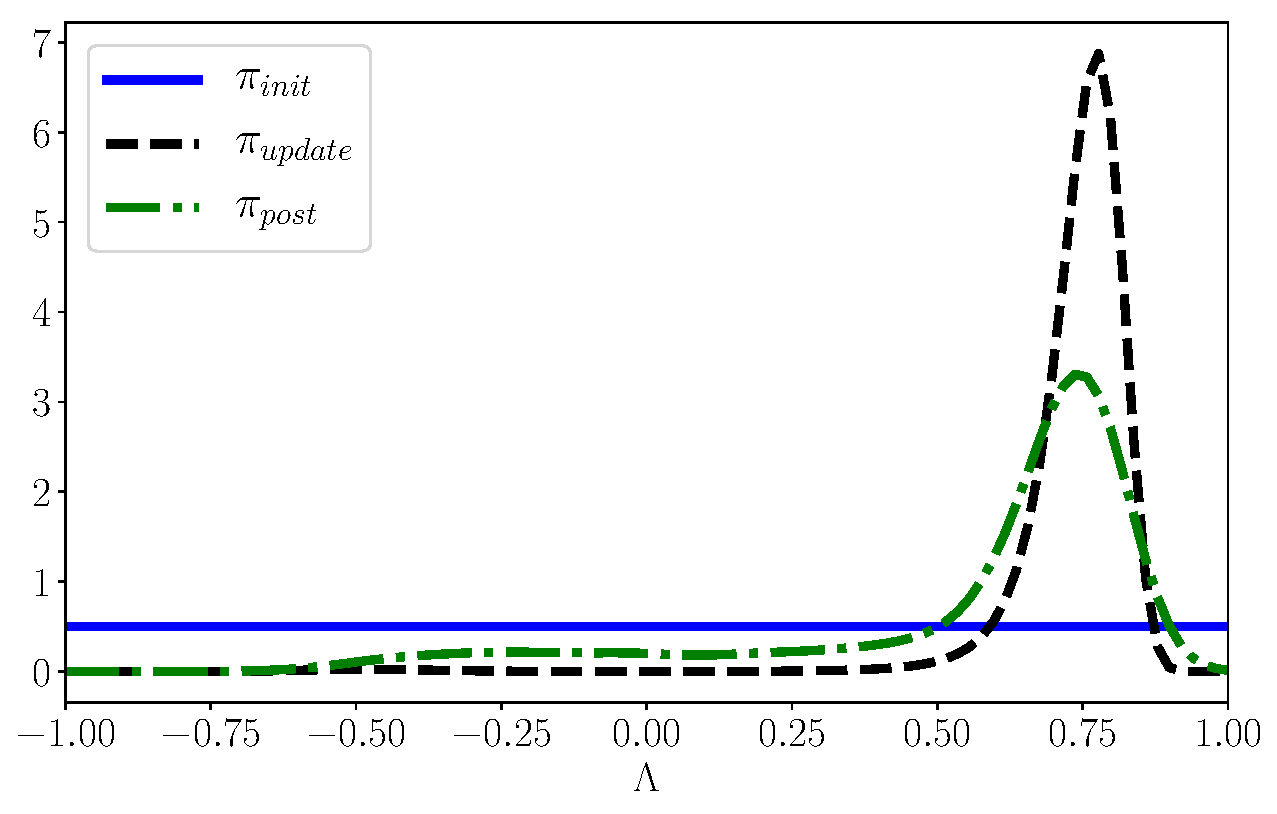
\includegraphics[width=0.49\linewidth]{figures/cbayes_comp_sbayes_50000_paramdens_nonlinear-standalone.pdf}
   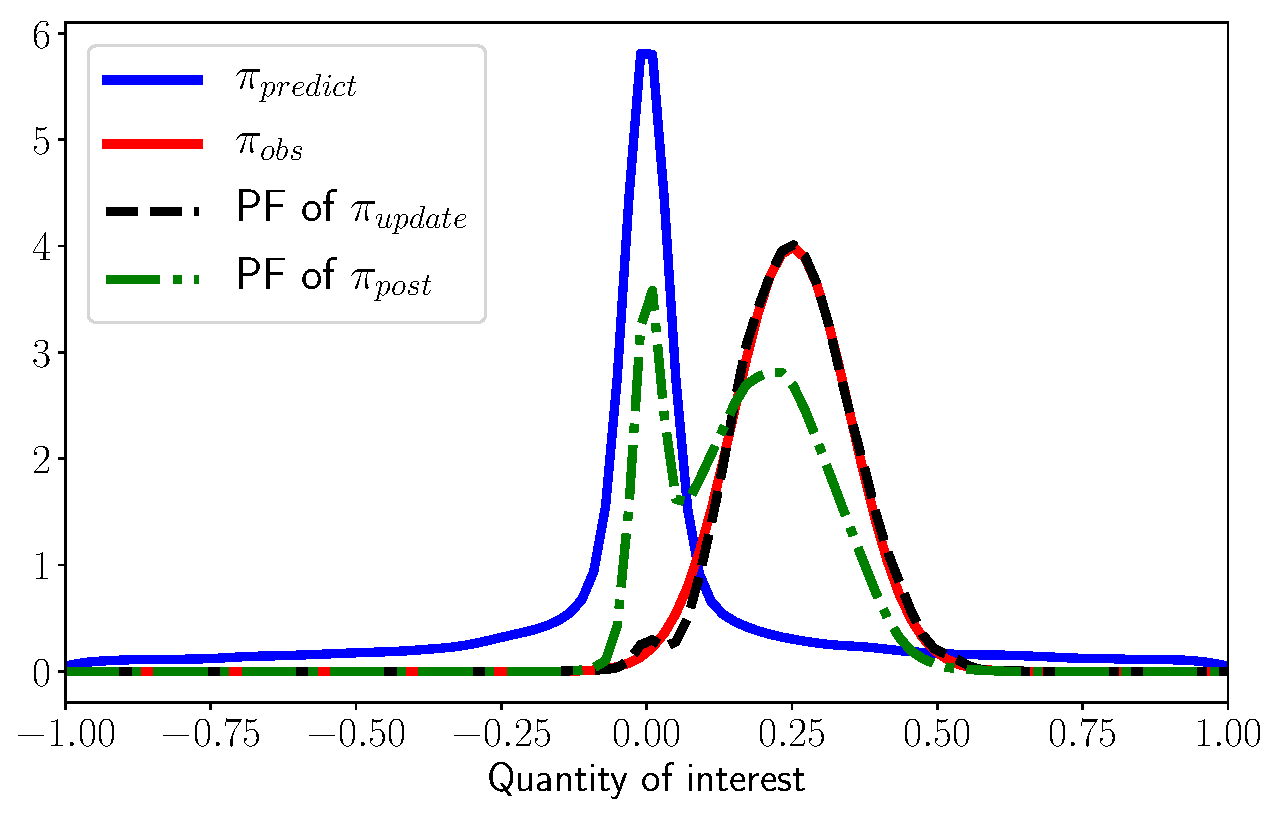
\includegraphics[width=0.49\linewidth]{figures/cbayes_comp_sbayes_50000_outdens_nonlinear-standalone.pdf}
 \caption{(Left) The initial/prior PDF $\initial$ (blue solid curve), updated PDF $\updated$ (black dashed curve), and posterior PDF $\pi_\text{post}$ (green dashed-dotted curve) on $\Lambda$.
 (Right) The push-forward (PF) of the initial/prior PDF $\predicted$ (blue solid curve), observed/likelihood PDF (red solid curve), PF of the updated PDF $\updated$ (black dashed curve), and the PF of the posterior PDF $\pi_\text{post}$ (green dashed-dotted curve) for the QoI.}
 \label{fig:bayes-comparison}
\end{figure}

The takeaway to the above discussion and example is that each density is solving a {\em different} inverse problem.
The posterior density is intended to provide point estimates of a true parameter value whereas the updated density is intended to quantitatively characterize natural variations in parameter values.

Suppose we reformulated this example slightly to make the role of data more central.
Specifically, suppose $Q(\paramref)=0.25$ and noisy measurement data are drawn from a $N(0.25,0.1^2)$, i.e., we assume that $d=Q(\paramref)+\xi$ where $\xi\sim N(0,0.1^2)$.
For the SIP, we could use the sample mean and variance of this data to estimate the ``exact'' observed $N(0.25,0.1^2)$ distribution whereas the data-likelihood would involve a product of normal densities.
In this case, the objective is to use the posterior or updated density to produce an estimate of $\paramref$.
In the next section, we motivate the use of the maximal updated density point as a means of providing a useful point estimate to parameters.


%A critical component in the Bayesian framework is the prior density, which encodes any knowledge or assumptions about them input (parameter) space that we may wish to impose before any data are observed.
%In some cases, the prior and initial densities may be both specified and interpreted identically.
%However, in the Bayesian framework, the impact of the prior on the posterior density is perhaps best understood as a regularization term that makes the inverse problem well--posed by penalizing parameters uninformed by the data.
%Ideally, the prior should not interfere with well--informed parameters, i.e., parameters informed by the data.
%{Unfortunately, well--informed parameters are not known a priori and none of the existing prior elicitation approaches avoid polluting data--informed directions in the parameter space.}





%%%%%%%%%%%%%%%%%%%%%%%%%%%%%%%%%%%%%%%%%%%%%%%%%%%%%%%%%%%%%%%%%%%%
%%%%%%%%%%%%%%%%%%%%%%%%%%%%%%%%%%%%%%%%%%%%%%%%%%%%%%%%%%%%%%%%%%%%
\section{Comparing the Maximal Updated Density (MUD) and MAP points}\label{sec:estimation}
%%%%%%%%%%%%%%%%%%%%%%%%%%%%%%%%%%%%%%%%%%%%%%%%%%%%%%%%%%%%%%%%%%%%
%%%%%%%%%%%%%%%%%%%%%%%%%%%%%%%%%%%%%%%%%%%%%%%%%%%%%%%%%%%%%%%%%%%%%%%%%%%%

We define the maximal updated density (MUD) point as
\begin{equation}\label{eq:mudpt_inital_defn}
	\mudpt := \argmax {\updated}(\param).
\end{equation}
We motivate the use of the MUD point as an alternative to a the MAP point for parameter estimation problems.
In this section, we assume linear (or affine) QoI maps with Gaussian distributions, which are often used in the UQ literature for providing a common framework for comparing methods and their solutions.

This section is structured into several subsections to help focus the interpretations and results.
In Section~\ref{subsec:Motivation}, we present some useful details, notation, and terminology used for this comparison framework.
To build intuition, we compare both the MUD and MAP points in Section~\ref{subsec:low-d-example} using a low-dimensional example.
A unifying perspective is provided for affine maps in Section~\ref{subsec:unifying-perspective} along with derivations of closed form expressions for the MUD and MAP points in this comparison framework.
These results are summarized in a theorem of existence and uniqueness of the MUD point in this comparison framework.
%Subsection~\ref{subsec:MUD-MAP-generalized-contours} provides some useful interpretations of the MUD and MAP points in terms of their connections to points on generalized contours and relationships to least-squares solutions.
%Finally, in Subsection~\ref{subsec:MUD-theorem}, we summarize the theory of existence and uniqueness for the MUD point.
%along with several numerical results that compare features of the MUD point to two other point estimates: the MAP point obtained from a Bayesian formulation and the solutions to a least-squares problem.


\subsection{MUD and MAP points for the ``linear Gaussian'' case}\label{subsec:Motivation}

%{\bf Regularization/deterministic optimization connections.
%The type of problem is now different involving parameter identification under uncertainty}


\begin{table}[htbp]
\centering
\begin{tabular}{|c|c|}
\hline
  & \\
  Tikhonov & $T(\param):=\norm{Q(\param)-\observedMean}_{\observedCov^{-1}}^2 +
      \norm{\param-\initialMean}_{\initialCov^{-1}}^2$
  \\ & \\ \hline & \\
  Data-Consistent & $J(\param):=T(\param) - \norm{Q(\param)-Q(\initialMean)}_{\predictedCov^{-1}}^2$
  \\ & \\
  \hline
\end{tabular}
\caption{Functionals to minimize to obtain $\param$ that maximizes  the updated PDF (left) and the Bayesian posterior PDF (right).
Here, $T(\param)$ is the typical functional often associated with Tikhonov regularization, and the $J(\param)$ has an additional term subtracted from $T(\param)$ coming from the predicted density that serves as ``unregularization'' in data--informed directions.}
  \label{tab:func_comparisons}
\end{table}

Let $\norm{\mathbf{x}}_C^2 := (\mathbf{x}, \mathbf{x})_C = \mathbf{x}^T C \mathbf{x} $ denote the square of the induced norm associated with a positive-definite operator $C : \RR^n \to \RR^n$ and the usual (Euclidean) inner product.
In what follows, the inverse covariances associated with non-degenerative multivariate Gaussian distributions will play the role of $C$.
%
%either attached to the Gaussian initial (prior) $\mathcal{N}(\param_0, \initialCov)$, observed $\mathcal{N}(\observedMean, \observedCov)$, or predicted $\mathcal{N}(Q(\param_0), \predictedCov)$ distributions.
%So, $C$ will play the roles of $\observedCov^{-1}$, $\initialCov^{-1}$, and $\predictedCov^{-1}$.

Suppose that both the initial and prior densities are both given by the same $\mathcal{N}(\param_0, \initialCov)$ distribution.
Additionally, suppose the map $Q$ is linear and that the data-likelihood and observed densities are both given by the same $\mathcal{N}(\observedMean, \observedCov)$ distribution.

The linearity of $Q$ implies that $Q(\param)=A\param$ for some $A\in\RR^{d\times p}$, and that the predicted density follows a $\mathcal{N}(Q(\param_0), \predictedCov)$ distribution where
\begin{equation}\label{eq:predictCov}
	\predictedCov := A\initialCov A^\top.
\end{equation}
While it is not technically necessary to ensure that the predictability assumption holds (i.e, that $\updated$ is in fact a density) in order to formally define a MUD point using~\eqref{eq:mudpt_inital_defn}, it is useful when discussing certain theoretical results involving data-constructed QoI maps as we see in Sections~\ref{subsec:unifying-perspective} and~\ref{sec:data-maps}.
%The predictability assumption holds whenever
%\begin{equation}\label{eq:predict_cov_assump}
%	\predictedCov \geq \observedCov,
%\end{equation}
%where the inequality is interpreted as holding term-wise.
%We therefore refer to the condition of~\eqref{eq:predict_cov_assump} as the predictability assumption for the linear Gaussian case.
Conceptually, the predictability assumption holds when the predicted variance is larger in all directions than the observed variance.
This condition is consistent with the desired outcome of a parameter estimation problem where the incorporation of observed data produces not only an improvement to the initial point estimate but also serves to reduce the uncertainty in this point estimate (quantified in this case by the covariance).
Mathematically, this occurs when the smallest eigenvalue value of $\predictedCov$ is larger than the largest eigenvalue value of $\observedCov$.

When $\observedCov$ is non-degenerative (i.e., the smallest eigenvalue is positive), the predictability assumption can always be satisfied if $d\leq p$ and $A$ is full rank by choosing $\initialCov$ to have sufficiently large eigenvalues (i.e., if we choose initial variances to be sufficiently large).
To simplify the theoretical presentation of this section, we assume these conditions are met so that the predictability assumption holds and $\updated$ does in fact define a density.
However, in Section~\ref{sec:high-dim-linear-example}, we still compute the formal MUD point for a high-dimensional example involving rank-deficient $A$ to demonstrate the overall usefulness of the MUD point even in situations where $\predicted$ may fail to be an actual density.

With these assumptions, the parameters that maximize the posterior and updated densities are easily described as the arguments that minimize certain quadratic functionals.
Specifically, Table~\ref{tab:func_comparisons} presents a scaling of these functionals defined by the negative logarithm of the associated posterior and updated densities.
Note that the functional, $T(\param)$, obtained from the posterior density is immediately identified as the typical functional used in Tikhonov regularization.
The data-mismatch term defined by
\begin{equation*}
	\norm{Q(\param)-\observedMean}_{\observedCov^{-1}}^2
\end{equation*}
comes from the data-likelihood/observed density whereas the regularization term defined by
\begin{equation*}
	 \norm{\param-\initialMean}_{\initialCov^{-1}}^2
\end{equation*}
comes from the prior/initial density.
We refer to this term as the Tikhonov regularization term.
However, the functional, $J(\param)$, obtained from the updated density is written as a modification of the $T(\param)$ function where the subtraction of
\begin{equation*}
	 \norm{Q(\param)-Q(\initialMean)}_{\predictedCov^{-1}}^2
\end{equation*}
comes from the {\em predicted} density.

\subsection{A low-dimensional example}\label{subsec:low-d-example}

To build intuition around the fundamental differences of MAP and MUD points, we consider an example where the linear QoI map is defined by $A=\mat{cc}{1 & 1}$, i.e., the parameter space is 2-dimensional while the data space is 1-dimensional.
The parameters in the initial and observed densities are given by
\[
	\initialMean = \mat{cc}{0.25 & 0.25}^\top, \initialCov = \mat{cc}{1 & -0.25 \\ -0.25 & 0.5}, \ \observedMean=1, \text{ and } \observedCov = \mat{c}{0.25}.
\]

\begin{figure}
   % 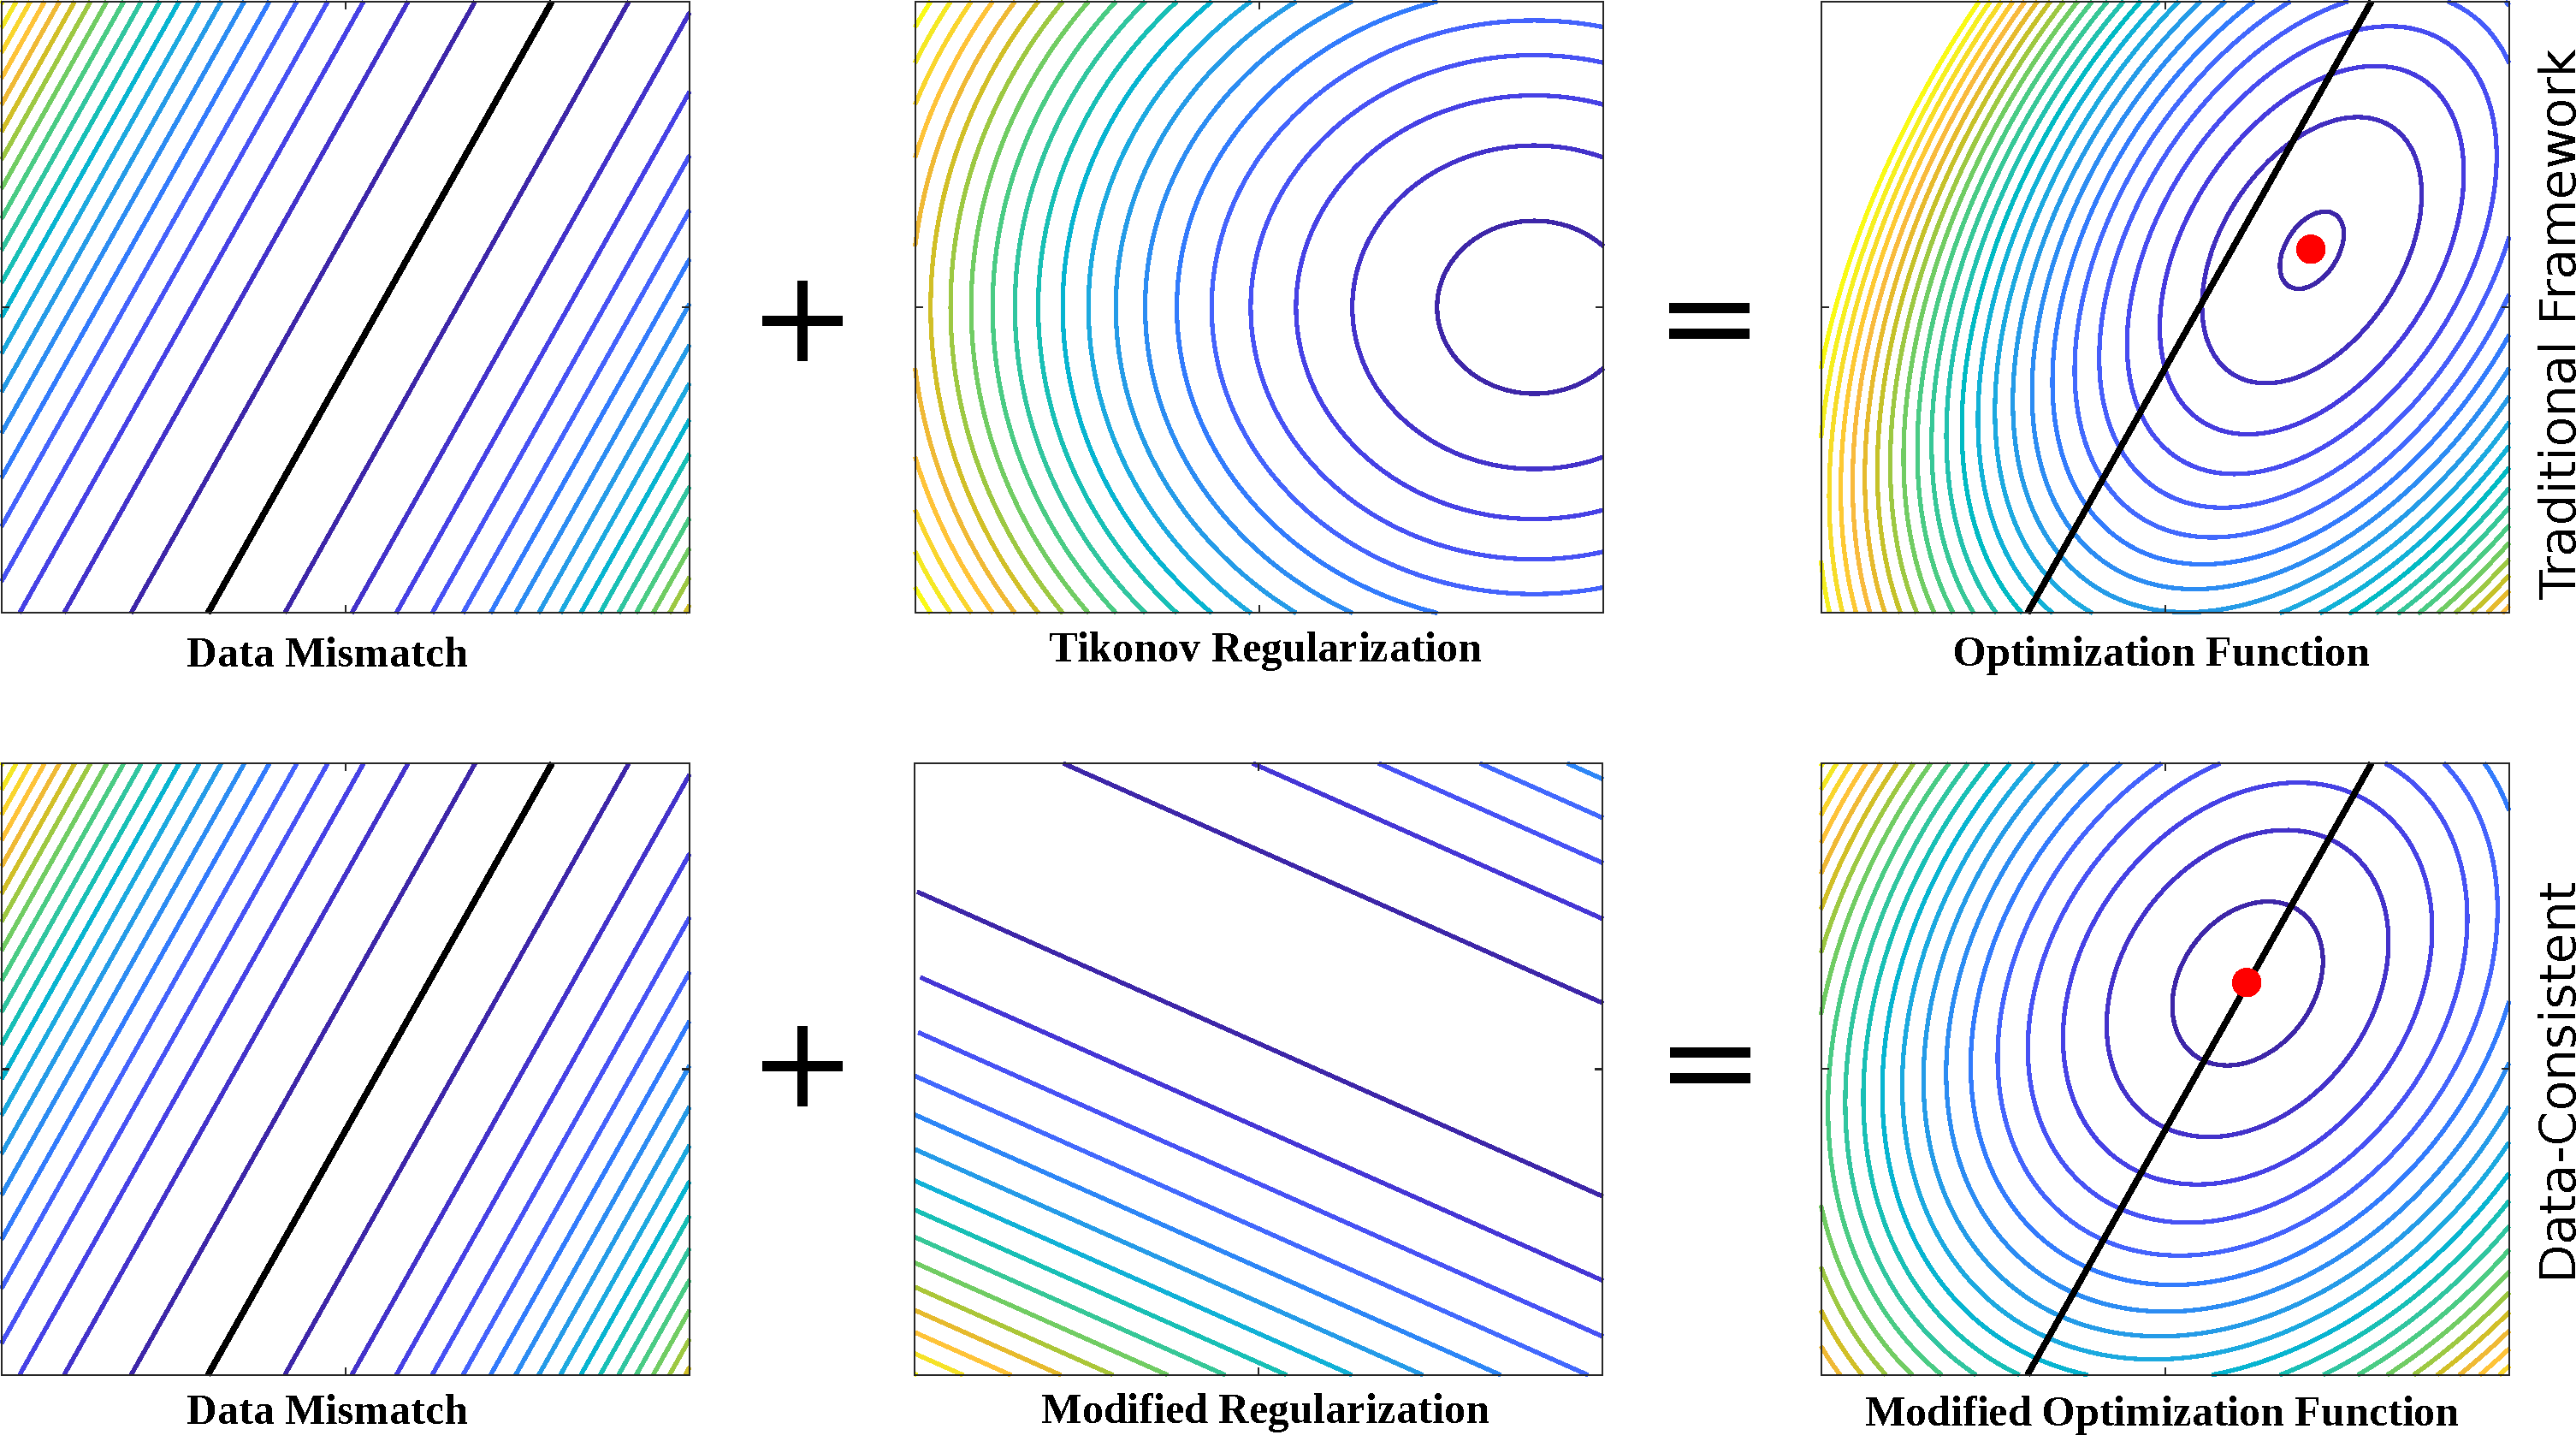
\includegraphics[width=\linewidth]{figures/Regularization-all-in-one.pdf}
  \centering
  \begin{tabular}{|ccc|}
    \hline
      \subf{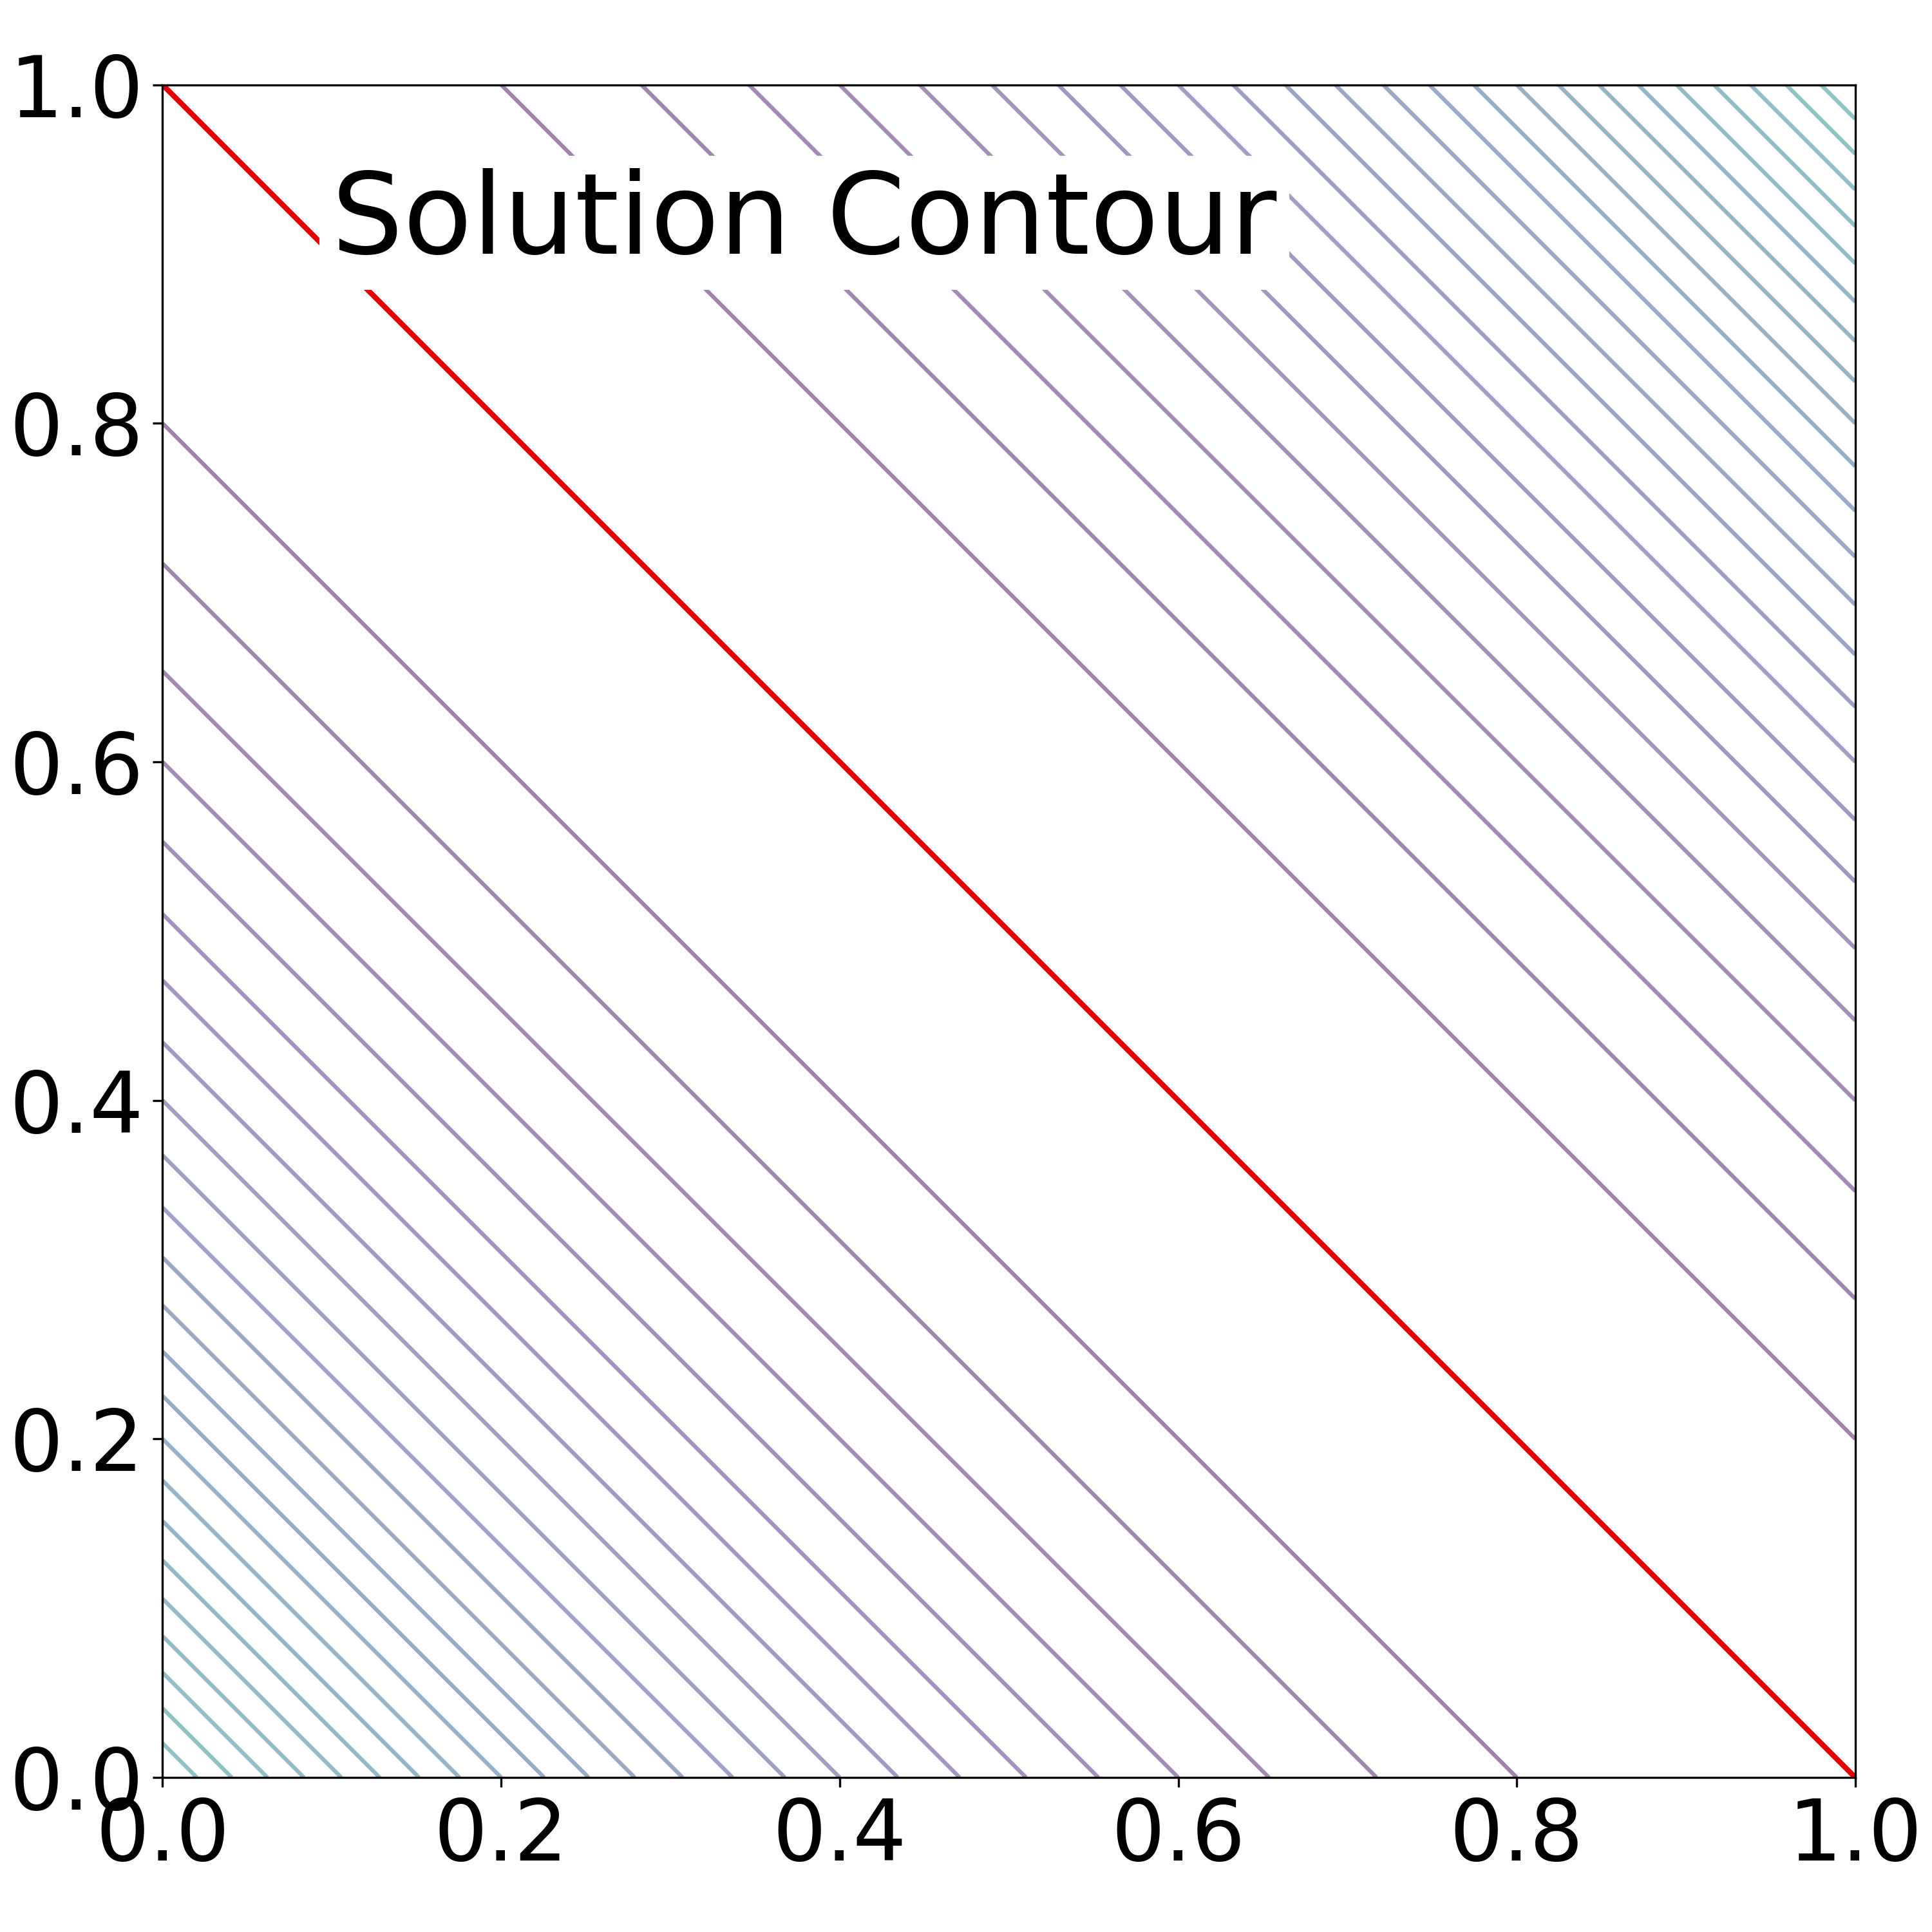
\includegraphics[width=0.3\linewidth]{figures/data_mismatch_contour.png}}
      {data mismatch}
    &
      \subf{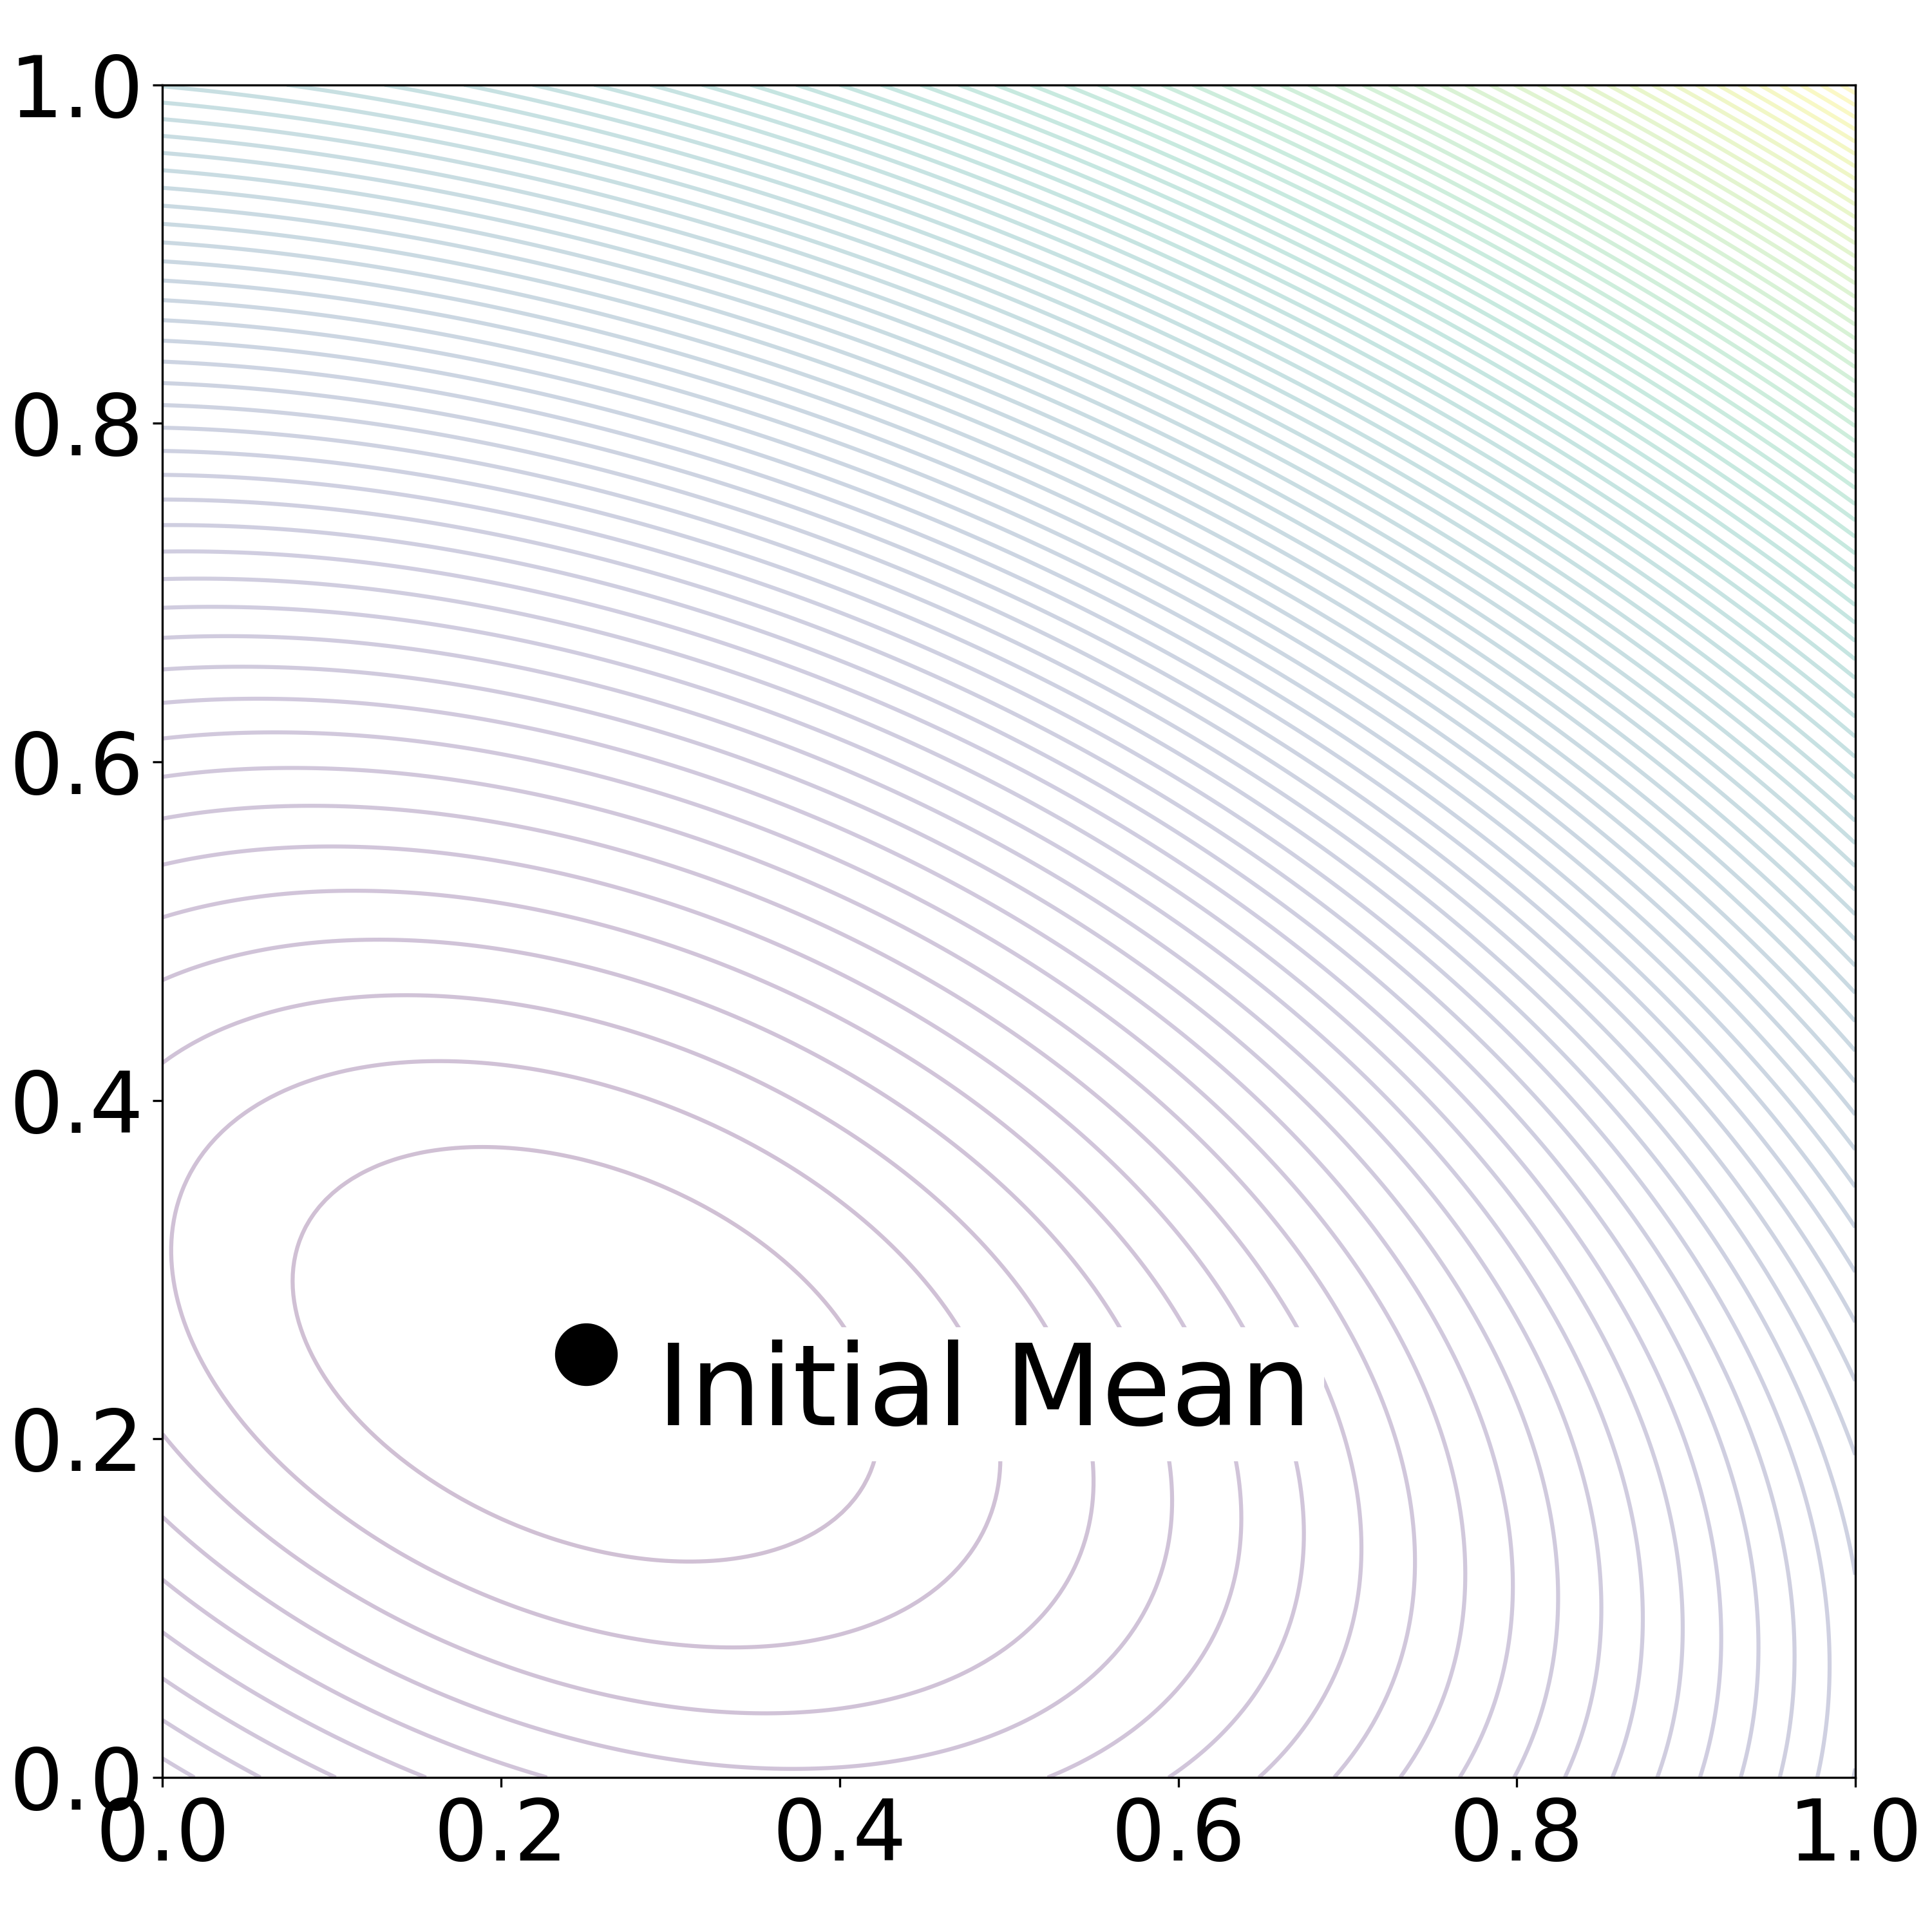
\includegraphics[width=0.3\linewidth]{figures/tikonov_contour.png}}
      {regularization}
    &
      \subf{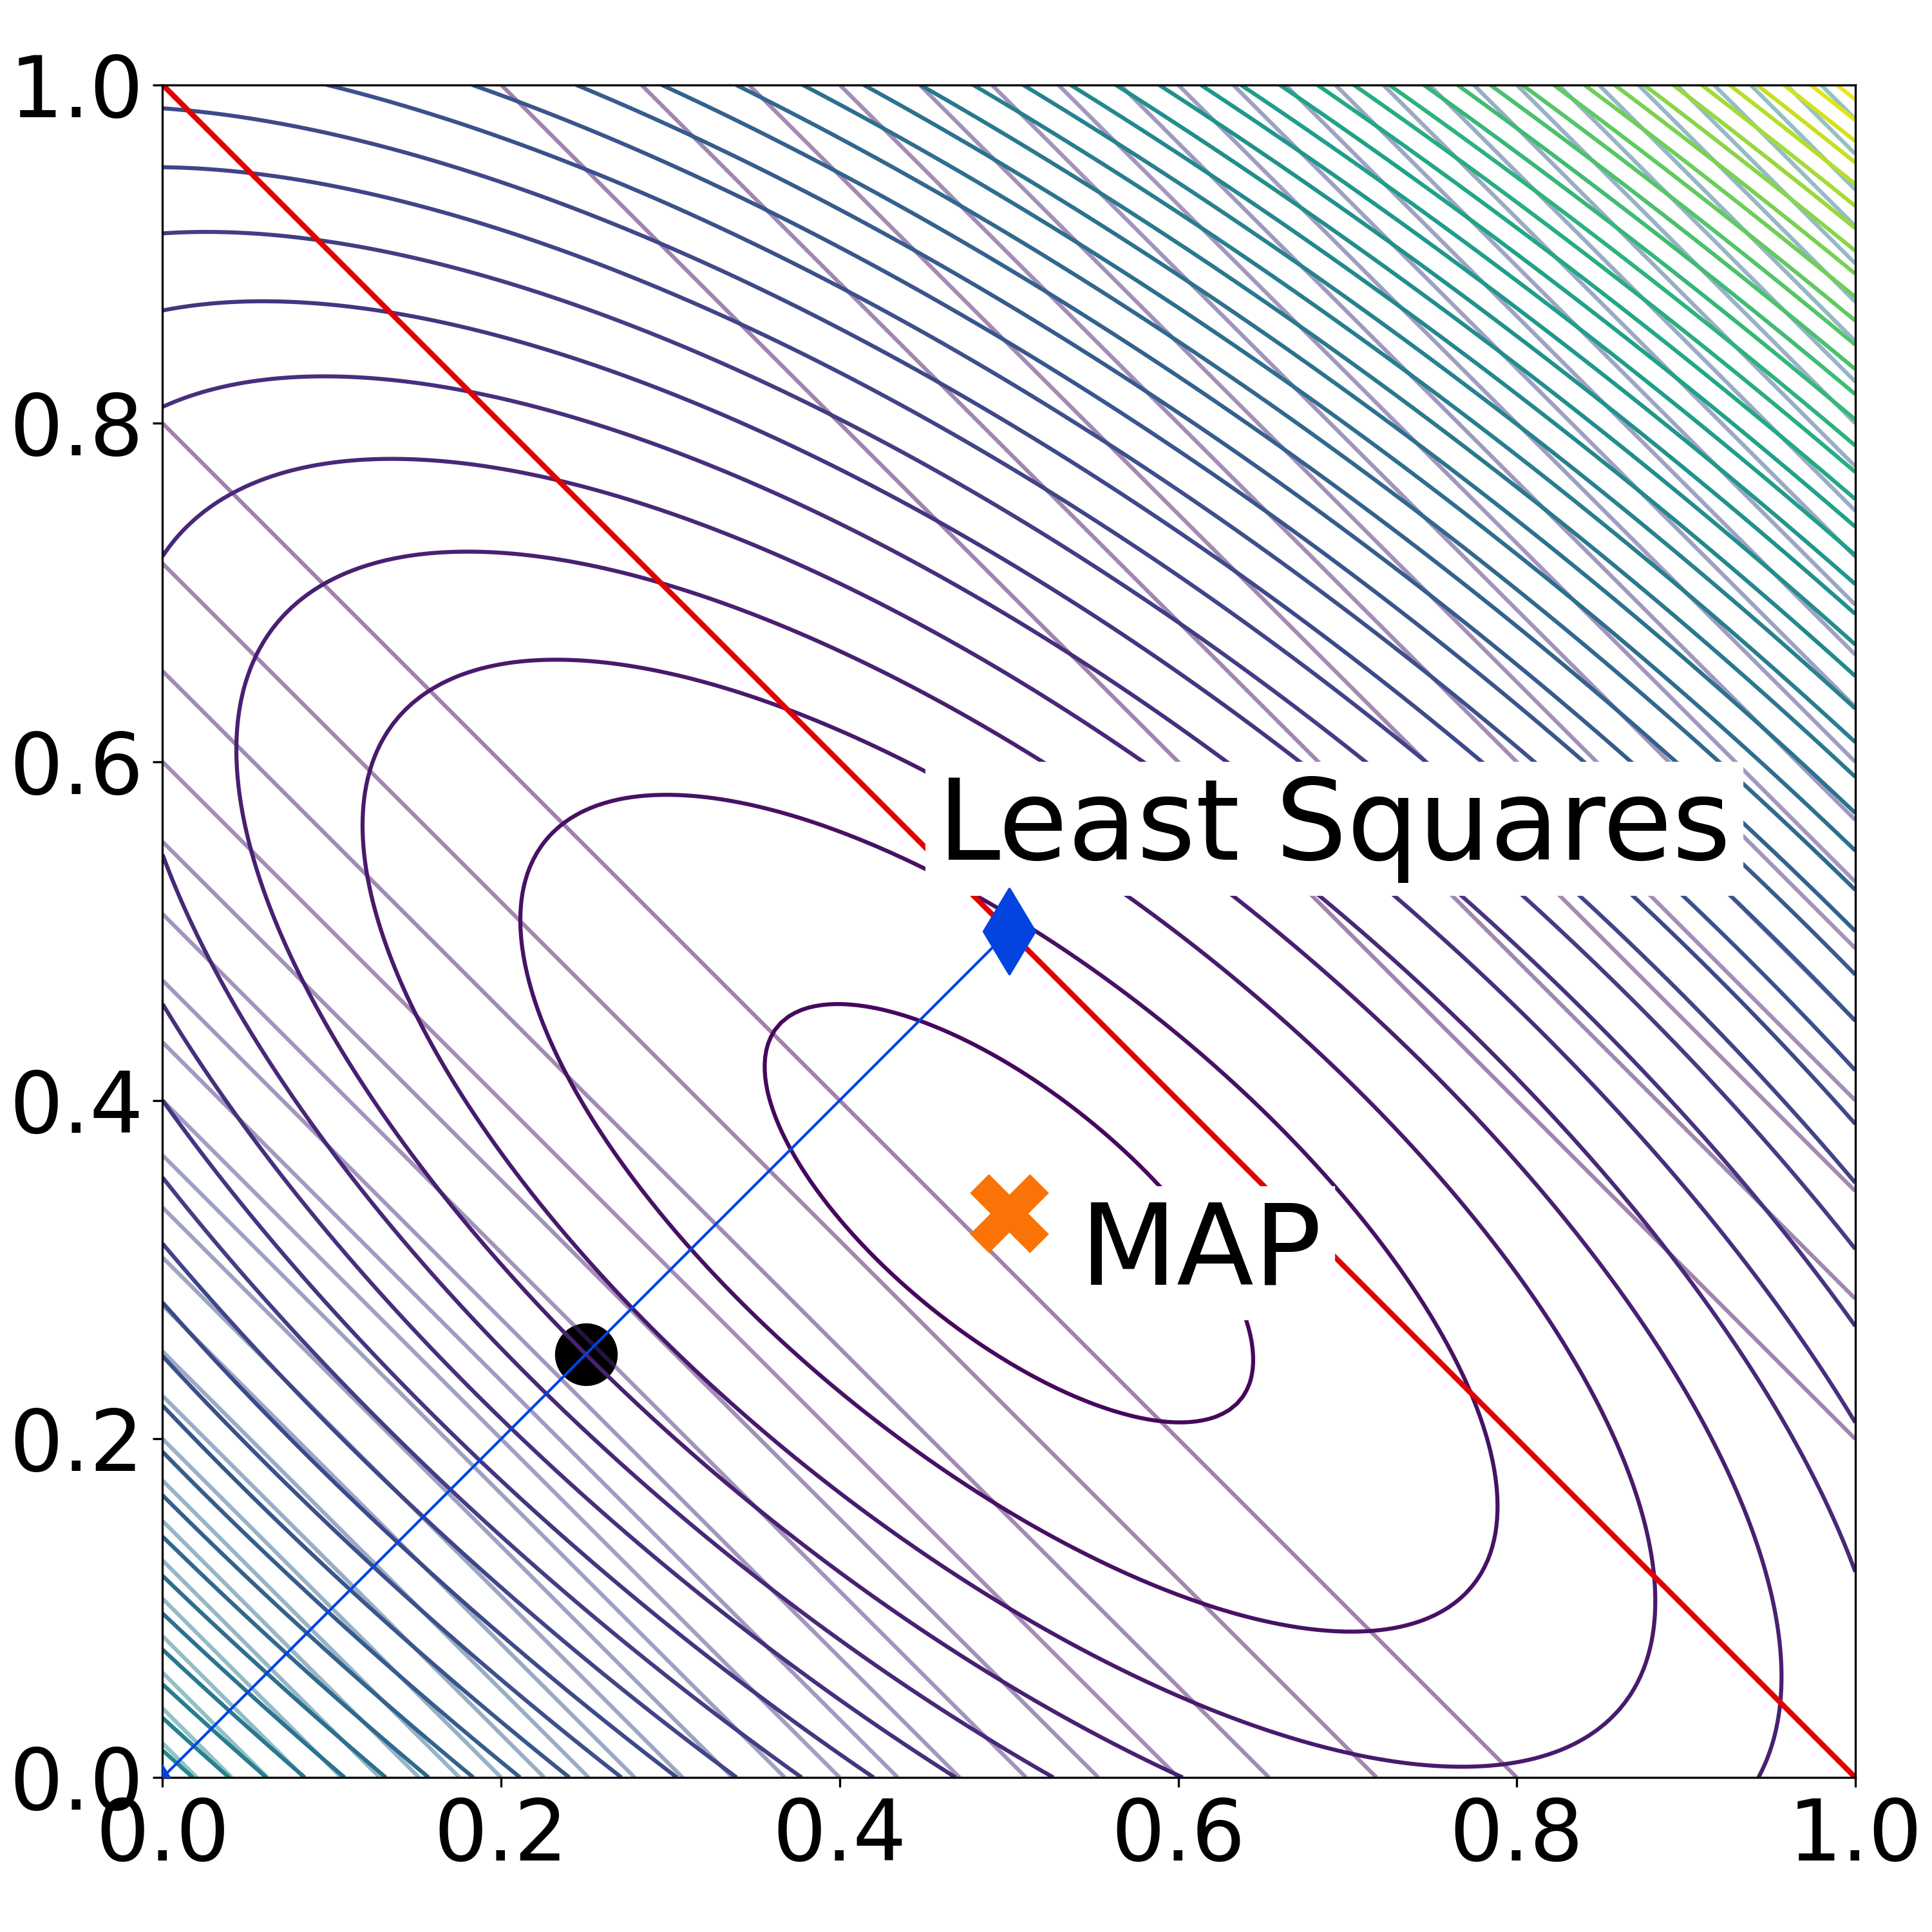
\includegraphics[width=0.3\linewidth]{figures/classical_solution.png}}
      {bayesian posterior}
    \\
    \hline
      \subf{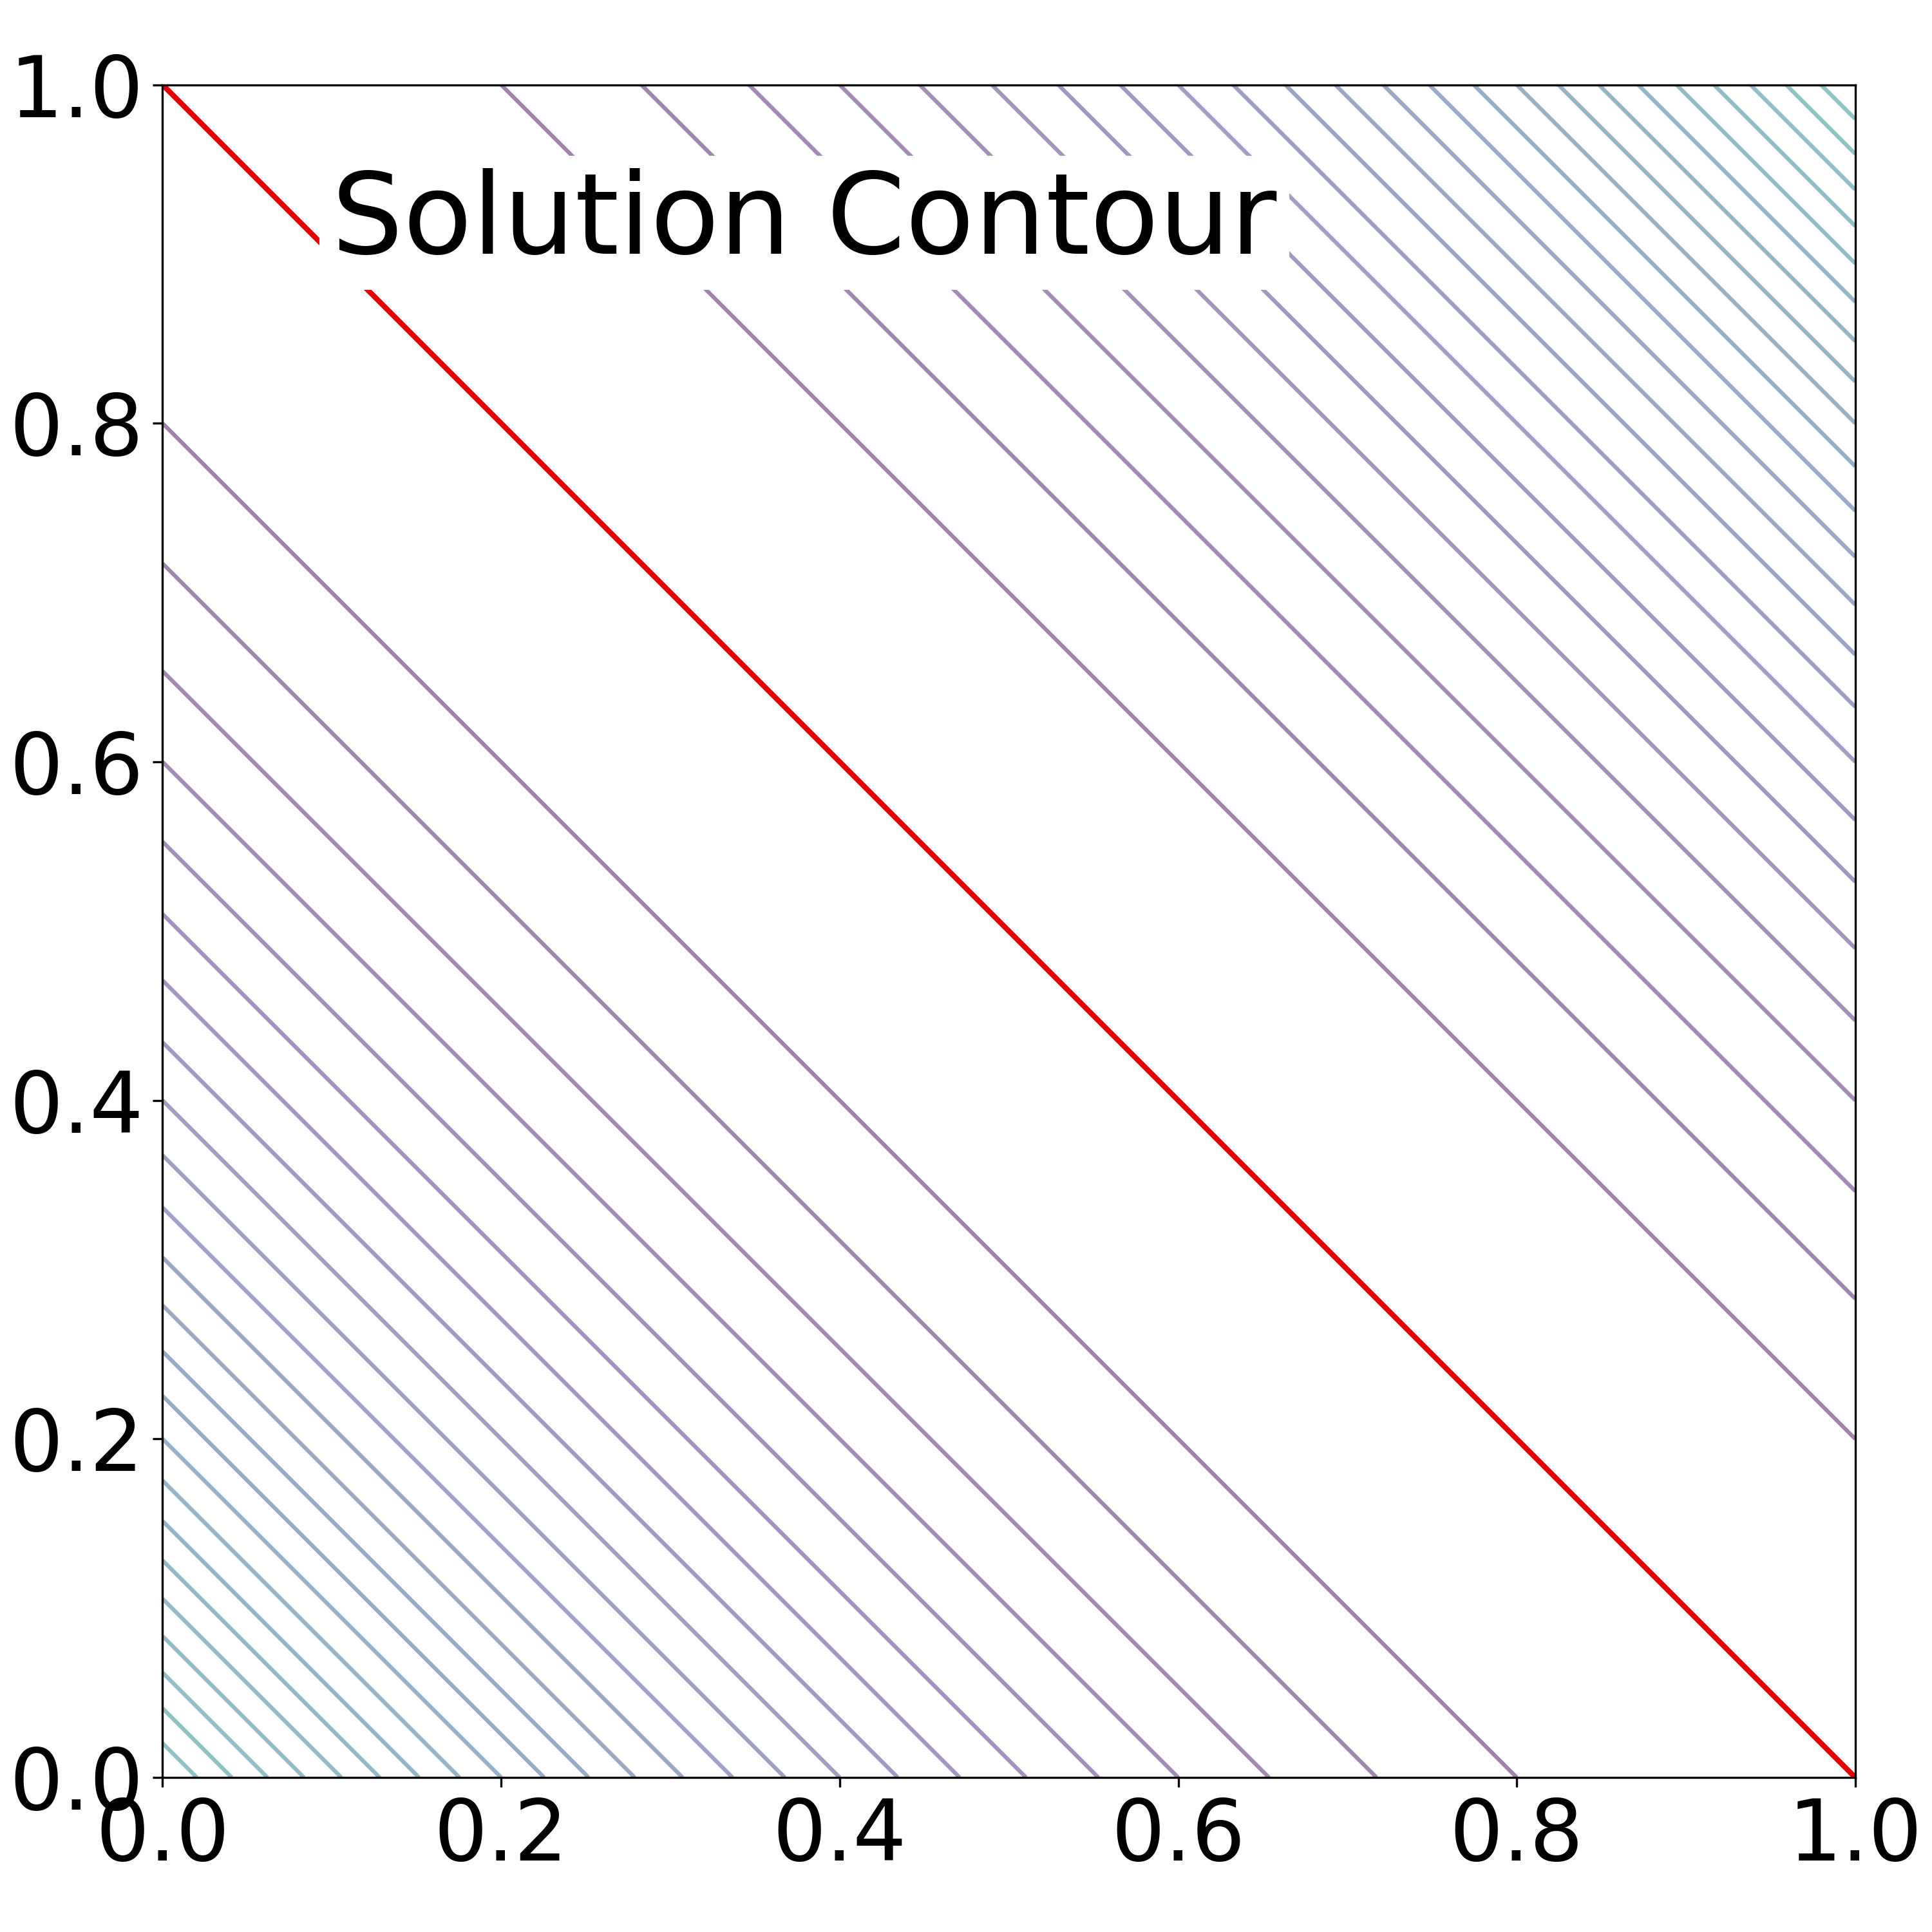
\includegraphics[width=0.3\linewidth]{figures/data_mismatch_contour.png}}
      {data mismatch}
    &
      \subf{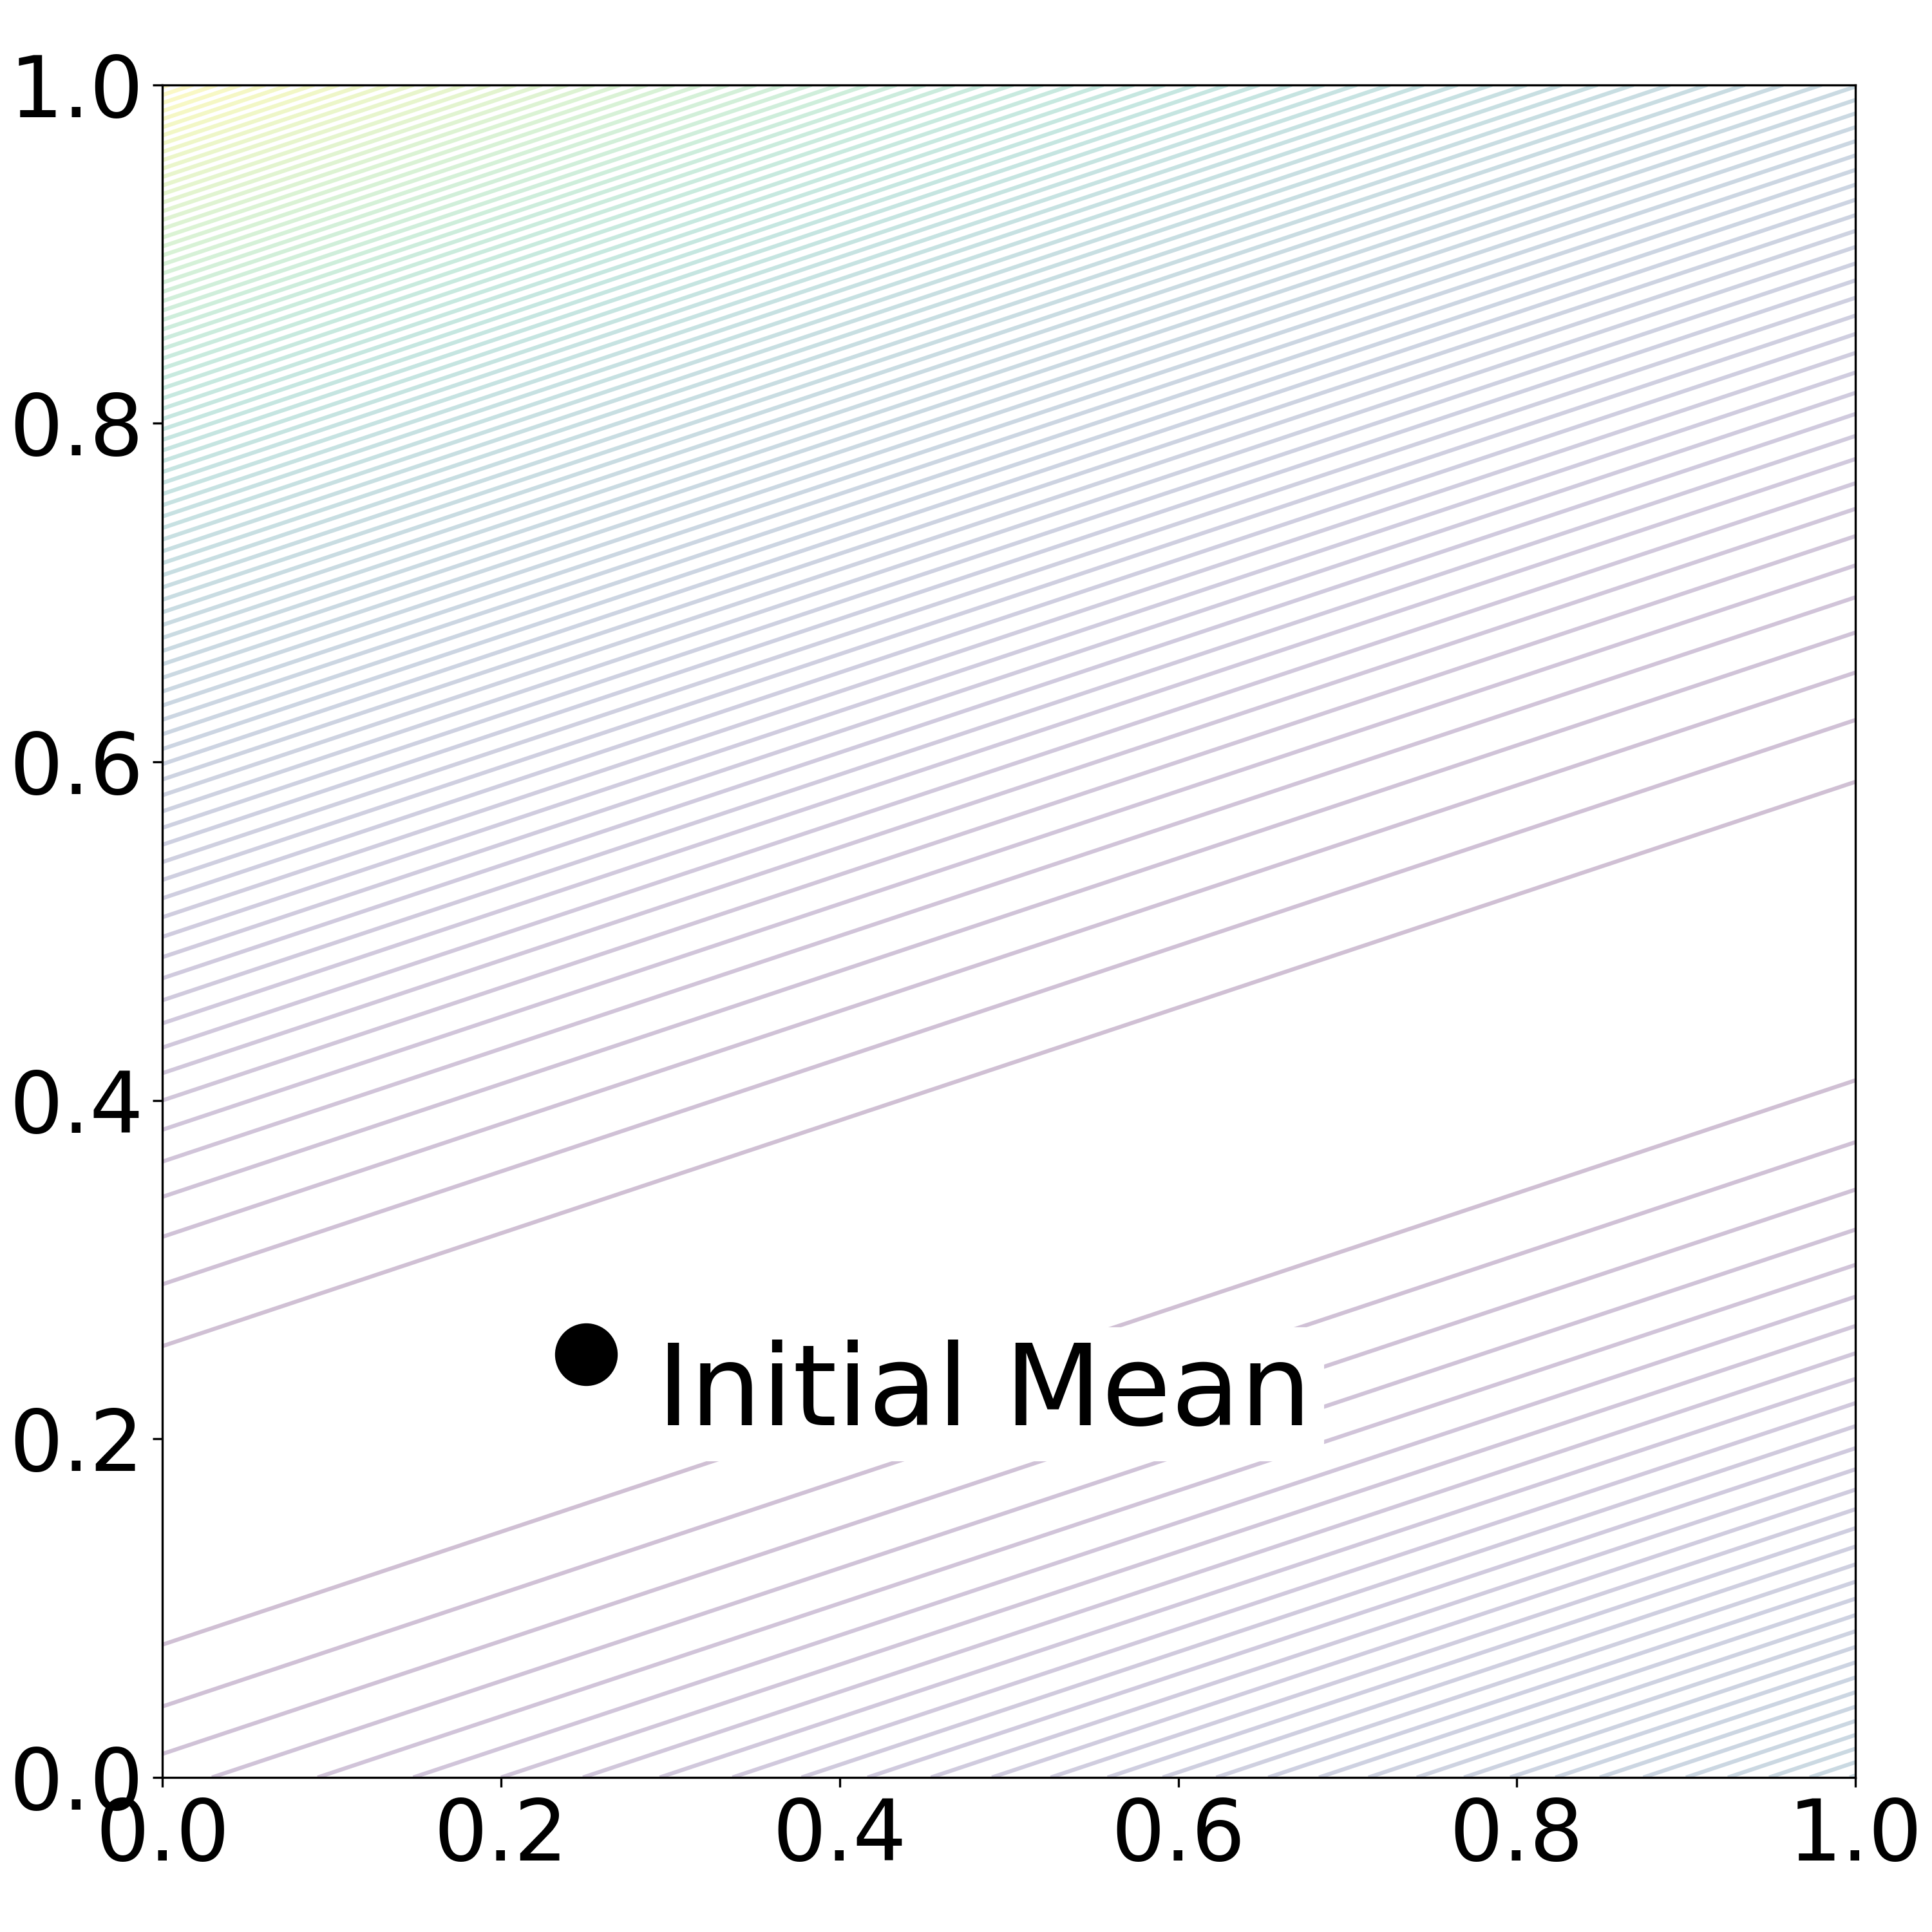
\includegraphics[width=0.3\linewidth]{figures/consistent_contour.png}}
      {modified regularization}
    &
      \subf{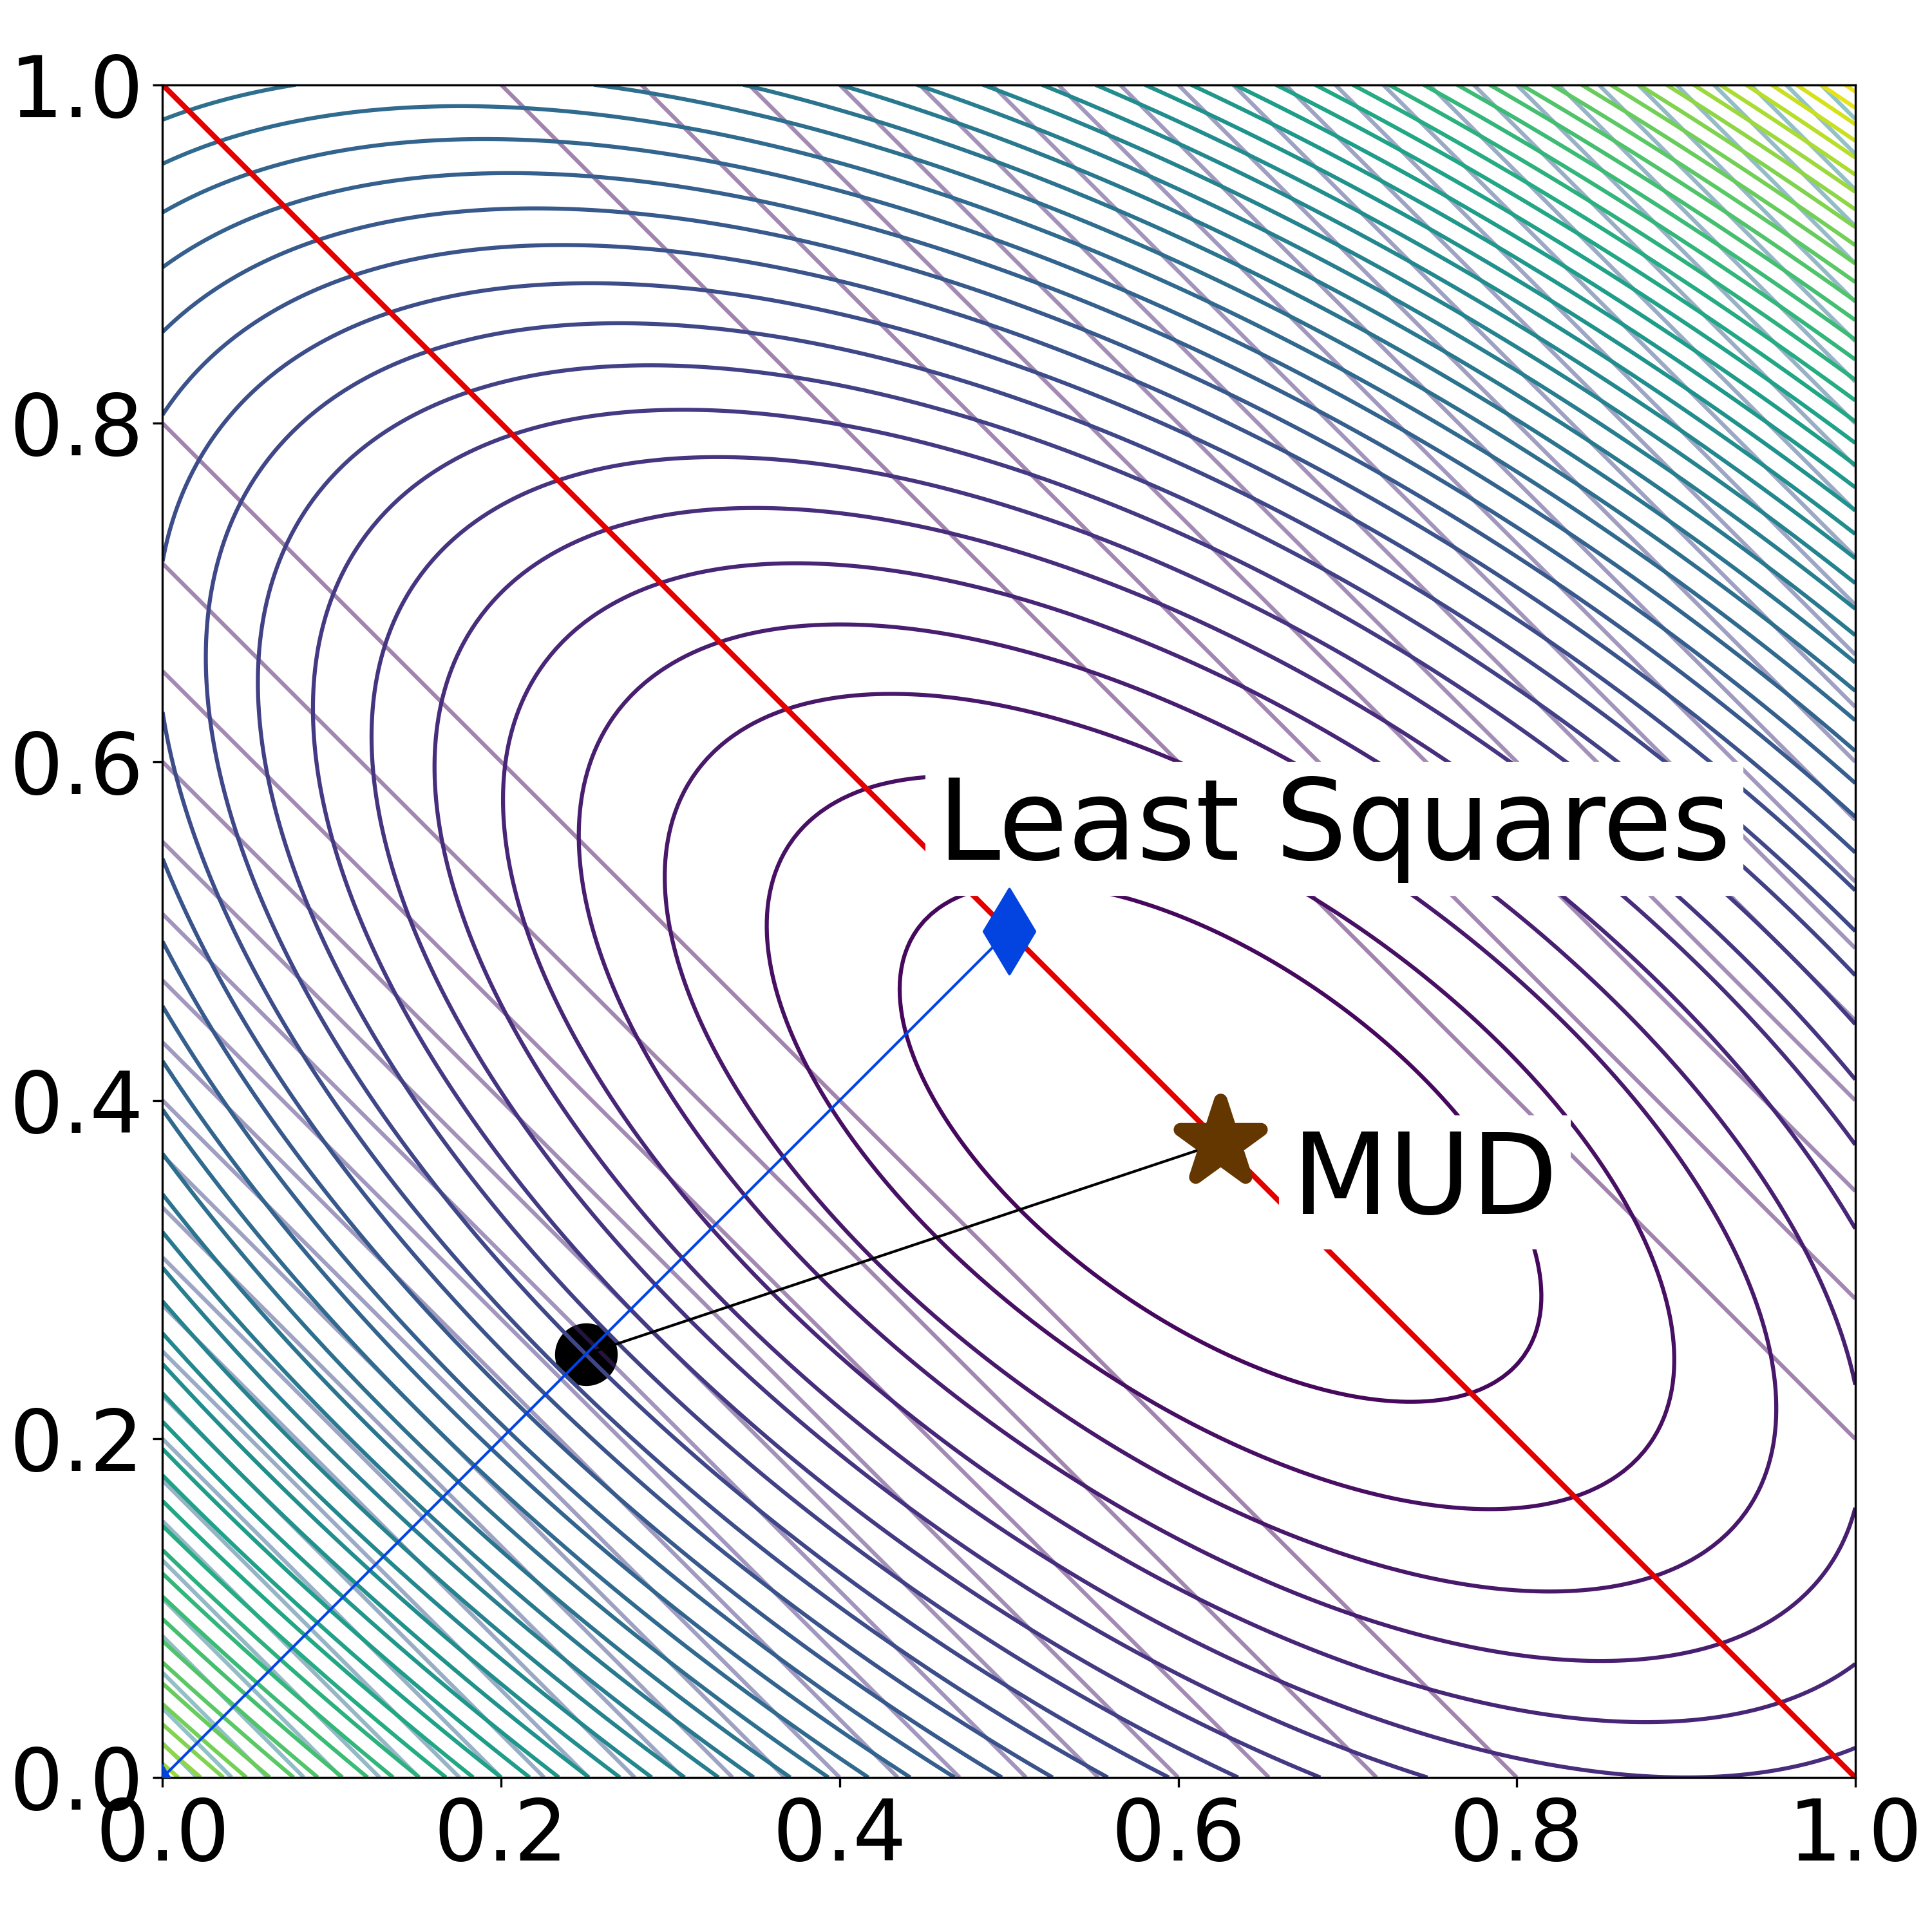
\includegraphics[width=0.3\linewidth]{figures/consistent_solution.png}}
       {updated density}
    \\
    \hline
  \end{tabular}

  \caption{Gaussian data mismatch over 2-D parameter space for a 2-to-1 linear map (left plots). Gaussian initial/prior lead to different regularization terms associated with updated/Bayesian PDFs (middle plots), which lead to different optimization functions (right plots) and parameter estimates that produce maximum PDF values for update/Bayesian PDF (red dot in right plots).}
  \label{fig:regularization}
\end{figure}


The top row of Fig.~\ref{fig:regularization} shows contour plots in the parameter space for the data-mismatch term (left), Tikhonov regularization term (middle), as well as the functional $T(\param)$ (right).
Conceptually, the regularization term is a radially symmetric function that penalizes parameters that are far away from the initial mean.

The bottom row of Fig.~\ref{fig:regularization} shows contour plots in the parameter space for the data-mismatch term (left), modified regularization term (middle), as well as the functional $J(\param)$ (right).
Here, we see that the modified regularization term only penalizes the movement of parameters in certain directions away from the initial parameter mean.

%%%%%%%%%%%%%%%%%%%%%%%%%%%%%%%%%%%%%%%%%%%%%%%%%%%%%%%%%%%%%%%%%%%%
%%%%%%%%%%%%%%%%%%%%%%%%%%%%%%%%%%%%%%%%%%%%%%%%%%%%%%%%%%%%%%%%%%%%

\subsection{A unifying perspective and closed form solutions}\label{subsec:unifying-perspective}

Assume that the QoI map, $Q$, now takes the slightly more general form
\begin{equation}\label{eq:qoi_map}
Q(\param) = A \param + \mathbf{b}
\end{equation}
where $\mathbf{b} \in \RR^d$ may be viewed as a bias in the QoI map.
The inclusion of this term makes is relevant for drawing conclusions involving the data-constructed QoI maps presented in Section~\ref{sec:data-maps}.
Using the same Gaussian distribution assumptions as described in Section~\ref{subsec:Motivation}, we again identify the MAP and MUD points as the values that minimize the functionals $T(\param)$ and $J(\param)$, respectively, shown in Table~\ref{tab:func_comparisons}.


The posterior covariance is formally given by
\begin{equation}\label{eq:map_cov}
\Sigma_\text{post} := ( A^\top {\Sigma}_\text{obs}^{-1} A + \initialCov^{-1} )^{-1}.
\end{equation}
Applying the Woodbury matrix identity and~\eqref{eq:predictCov}, we rewrite the posterior covariance as
\begin{equation}\label{eq:map_cov_analytical}
\Sigma_\text{post} = \initialCov - \initialCov A^\top \left[\predictedCov + \observedCov\right]^{-1} A \initialCov,
\end{equation}
which allows us to interpret $\Sigma_\text{post}$ as a rank $d$ correction (or update) of $\initialCov$.
Note that $\predictedCov + \observedCov$ is invertible because it is the sum of two symmetric positive definite matrices.
With either version of $\Sigma_\text{post}$ given above, we rewrite the closed form expression for the MAP poing given in \cite{Tarantola_book} as
\begin{equation}\label{eq:map-point-analytical}
\param^{\text{MAP}} = \param_0 + \Sigma_\text{post} A^\top \observedCov^{-1} (\observedMean - b - A\param_0).
\end{equation}
%where the posterior covariance is given by
%\begin{equation}\label{eq:map_cov}
%\Sigma_\text{post} = ( A^\top {\Sigma}_\text{obs}^{-1} A + \initialCov^{-1} )^{-1},
%\end{equation}
%which is


We now derive an alternative representation of $J(\param)$ to draw comparisons to the posterior covariance and MAP point.
First, define
\begin{equation}\label{eq:eff_reg}
	R := \nolinebreak \initialCov^{-1} - \nolinebreak A^\top \predictedCov^{-1} A.
\end{equation}
Using this $R$, rewrite $J(\param)$ as
\begin{equation}\label{eq:dci-objective-alt}
J(\param):= \norm{\observedMean - Q(\param)}_{\observedCov^{-1}}^2 + \norm{\param - \param_0}_{R}^2.
\end{equation}
In this form, we identify $R$ as the {\em effective regularization} in $J(\param)$ due to the formulation in the observation-consistent framework.


Observe that if $d=p$, then, by the assumption that $A$ is full-rank, $A$ is invertible.
In this case, $R$ is the $p\times p$ zero matrix and~\eqref{eq:dci-objective-alt} reduces to the data-discrepancy term so that the MUD point is recognizable as the least squares solution, i.e., the point that minimizes the data-discrepancy term.
Moreover, in this case we can immediately identify that $\mudpt = A^{-1}(\observedMean-b)$.
This is also evident from the perspective of the densities.
Specifically, in this case, $\updated$ is defined by applying a change of variables formula to $\observed$.
%Subsequently, the MUD point corresponds exactly to the point that maximizes $\observed$.

Suppose instead that $d<p$ so that the inverse-problem is under-determined.
In this case, we observe that constructing $R$ only requires specification of the initial/prior density and the QoI map, i.e., $R$ may be defined prior to any collection of data on the QoI.
Subsequently, we can interpret $J(\param)$ as coming from a modified Bayesian inverse problem with a prior defined by a $N(\param_0,\Sigma_R)$ distribution where $\Sigma_R=R^{-1}$.
In other words, the MUD and MAP points can both be interpreted as solutions to different Bayesian inverse problems.

However, $\Sigma_R$ is in fact a degenerative covariance, i.e., $R$ is not technically invertible.
This implies that $\Sigma_R$ cannot be directly substituted in for $\initialCov$ in~\eqref{eq:map_cov_analytical} to define a closed form expression for $\updatedCov$.
We therefore first substitute  $\Sigma_\text{post}$ and $\initialCov^{-1}$ in~\eqref{eq:map_cov_analytical} with $\updatedCov$  and $R$, respectively, to get
\begin{equation}
	\updatedCov := \left(A^\top \observedCov^{-1} A + R\right)^{-1}.
\end{equation}
Since $R$ is not invertible, Woodbury's identity cannot be applied (yet).
Using~\eqref{eq:eff_reg}, we rewrite this as
\begin{equation}
	\updatedCov = \left(A^\top \observedCov^{-1} A +  \initialCov^{-1} - \nolinebreak A^\top \predictedCov^{-1} A\right)^{-1},
\end{equation}
which is re-arranged as
\begin{equation}
	\updatedCov = \left(A^\top \left[\observedCov^{-1} - \predictedCov^{-1}\right]A + \initialCov^{-1}\right)^{-1}.
\end{equation}
Recall from Section~\ref{subsec:Motivation} that the predictability assumption in this case is that the smallest eigenvalue of $\predictedCov$ is larger than the largest eigenvalue of $\observedCov$.
The roles are reversed when we consider the inverses of these matrices.
Subsequently, $\observedCov^{-1}-\predictedCov^{-1}$ is a symmetric positive definite matrix and thus invertible.
Applying the Woodbury identity yields
\begin{equation}\label{eq:updated_cov_almost}
	\updatedCov = \initialCov - \initialCov A^\top\left( \left[\observedCov^{-1} - \predictedCov^{-1}\right]^{-1} + \predictedCov\right)^{-1} A\initialCov.
\end{equation}
Applying Hua's identity and simplifying gives
\begin{equation}\label{eq:Hua}
	\left( \left[\observedCov^{-1} - \predictedCov^{-1}\right]^{-1} + \predictedCov\right)^{-1} = \predictedCov^{-1}\left[\predictedCov - \observedCov\right]\predictedCov^{-1}.
\end{equation}
Substituting~\eqref{eq:Hua} into~\eqref{eq:updated_cov_almost} gives
\begin{equation}\label{eq:updatedCov_final}
	\updatedCov = \initialCov - \initialCov A^\top \predictedCov^{-1}\left[\predictedCov-\observedCov\right]\predictedCov^{-1}A\initialCov.
\end{equation}
We can now modify the expression for the MAP point given in~\eqref{eq:map-point-analytical} by substituting $\updatedCov$ for $\Sigma_\text{post}$ to write the MUD point that minimizes $J$ as
\begin{equation}\label{eq:mud-point-analytical-alt}
\param^{\text{MUD}} = \param_0 + \updatedCov A^\top \observedCov^{-1} (\observedMean - b - A\param_0).
\end{equation}
Substituting~\eqref{eq:updatedCov_final} into~\eqref{eq:mud-point-analytical-alt} and simplifying, we have
\begin{equation}\label{eq:mud-point-analytical-final}
	\mudpt = \param_0 + \initialCov A^\top \predictedCov^{-1}(\observedMean - b - A\param_0).
\end{equation}

Comparing~\eqref{eq:mud-point-analytical-final} to~\eqref{eq:map-point-analytical}, we
see that the MUD point does not depend on the observed covariance whereas the MAP point does.
%Both $\updatedCov$ and $\Sigma_\text{post}$ depend on $\observedCov$.
%Conceptually, this implies that the MUD point is not directly sensitivity to the amount of noise in observational data, but the noise directly impacts $\updatedCov$ in the data-informed directions.
%However, when $\observedMean$ is estimated by noisy data, this will impact the MUD and MAP points in similar ways.
Moreover, applying $Q$ to \eqref{eq:mud-point-analytical-final} and substituting accordingly reveals that $Q(\mudpt) = \observedMean$.

Overall, this motivates the MUD point as an \emph{alternative parameter estimate} with predictive accuracy and properties directly correlated to the relationship between $\observedMean$ and the true signal for which noisy data are generated.

These ideas are explored further in Section~\ref{sec:high-dim-linear-example} and utilized in the analysis of QoI maps constructed from noisy measurement data associated with a true parameter value in Section~\ref{sec:data-maps}.
We end this section by summarizing the above results in the following theorem stating the existence and uniqueness of a MUD point for the linear Gaussian case.

\begin{thm}\label{thm:MUD_existence_uniqueness}
Suppose  $Q(\param)=A\param+b$ for some full rank $A\in\RR^{d\times p}$ with $d\leq p$ and $b\in\RR^d$.
If $\initial \sim N(\param_0,\initialCov)$, $\observed\sim N(\observedMean,\observedCov)$, and the predictability assumption holds, then
\begin{enumerate}[(a)]
\item There exists a unique parameter, denoted by $\mudpt$, that maximizes $\updated$.
\item $Q(\mudpt) = \observedMean$.
\item If $d=p$, $\mudpt$ is given by $A^{-1}$. If $d<p$, $\mudpt$ is given by~\eqref{eq:mud-point-analytical-final} and the covariance associated with this point is given by~\eqref{eq:updatedCov_final}.
\end{enumerate}
\end{thm}



%%%%%%%%%%%%%%%%%%%%%%%%%%%%%%%%%%%%%%%%%%%%%%%%%%%%%%%%%%%%%%%%%%%%
\FloatBarrier
%%%%%%%%%%%%%%%%%%%%%%%%%%%%%%%%%%%%%%%%%%%%%%%%%%%%%%%%%%%%%%%%%%%%

\section{Higher-Dimensional Linear Gaussian Examples}\label{sec:high-dim-linear-example}

%For under-determined QoI maps, $\paramref$ is un-recoverable due to the set-valued nature of the set $Q^{-1}(\observedMean)$.
%While the incorporation of prior beliefs through the use of an initial or prior density allows us to determine a single ``best'' estimate of $\paramref$, this is not necessary.
%For instance, the least squares (LS) solution produces a single point estimate of $\paramref$ by enforcing a requirement of minimal norm.
%The LS solution will lie at the intersection of hyper-balls centered at the origin and the set-valued hyperplanes associated with $Q^{-1}(\observedMean)$, which is visible in Figure~\ref{fig:regularization} in 2-dimensions.

%By contrast, the Tikhonov-regularized solution selects a point that is biased by an initial covariance on $\Lambda$.
%The observation-consistent solution is an update to the initial mean in this same direction but always lies on the contour $Q^{-1}(\observedMean)$.
%The trouble is, none of these regularization approaches actually guarantee that in under-determined problems, the unique solutions that are selected are close to $\paramref$.

%There may or may not be good reasons for us to impose a requirement on the norm of the solution.
%If there are physical reasons relating to the magnitude of parameters involved, then the least-squares solution may very well be more accurate than the other two.
%However, not every problem lends itself to such structure.
%By contrast, if the initial beliefs are well-informed by the experience of the modeling team, it is possible that the MUD or MAP point out-perform Least-Squares.
%In situations where the beliefs are already really good (the mean is near the true value), and the data is really bad, the MAP solution may (by design) out-perform the MUD solution.
%If some beliefs are correct but others are not (the covariance incorporates some incorrect directions), the MUD point may dramatically out-perform the MAP point, especially in situations with few available measurements and strongly-held initial beliefs.

%Below we demonstrate with a pair of complementary examples involving linear maps which leverage the analytical equations presented in the previous section.
%We show that regardless of how well-informed your beliefs are, the convergence rate of the MUD solutions as more data is incorporated\---either by dimension or rank)\---will match those of the Least-Squares solutions.
%Moreover, the MUD solutions are not sensitive to scaling of the initial covariance (how strongly initial beliefs are held), the way that the MAP solution is.
%This provides a strong motivating factor for the consideration of the observation-consistent approach within the standard set of solution methods available to scientists and modelers who seek to perform parameter-identification.

%\subsection{MUD and MAP points and generalized contours}\label{subsec:gen_contours}

We first describe the relationship of MUD, MAP, and least squares estimates to the set-valued inverses of $Q$ in order to establish a conceptual framework for interpreting the numerical results that follow.
While this discussion is somewhat abstract, we refer to Figure~\ref{fig:regularization} to make these ideas more clear.

The MUD point exists on the generalized contour\footnote{We say generalized contour in this case because if $A$ is a $p$-to-$d$ full rank linear map with $d<p$, then $Q^{-1}(\observedMean)$ exists as a $(p-d)$-dimensional linear hyperplane in $\pspace$.} defined by $Q^{-1}(\observedMean)$.

This means that the MUD point retains the ``predictive precision'' of a least squares solution to the inverse problem (i.e., a parameter that minimizes the data-mismatch term $\norm{\observedMean - Q(\param)}_{\observedCov^{-1}}^2$) while incorporating the flexibility of prior beliefs in directions not informed by the QoI.
This is illustrated in the bottom right plot of Figure~\ref{fig:regularization}.
For under-determined or ill-conditioned problems, this suggests that ``good'' prior beliefs may be used to produce a MUD point that is more accurate than a least squares solution.
This is explored in the following examples involving high-dimensional linear maps.

By contrast, the MAP point exists on a line connecting the initial mean, $\param_0$, and the generalized contour defined by $Q^{-1}(\observedMean)$.
Substituting \eqref{eq:map_cov_analytical} into \eqref{eq:map-point-analytical}, we see that this line is in the direction of the orthogonal nullspace of the image of $A$ under $\initialCov$; i.e., $\mathcal{N}(\initialCov A)^\perp$.
In fact, this line intersects the generalized contour defined by $Q^{-1}(\observedMean)$ precisely at the MUD point.
If one parameterizes the line between $\param_0$ and $\param^{\text{MUD}}$, then one can also identify $\param^{\text{MAP}}$ as a convex sum of these two points.
The weights of this convex sum, which determine the position of the MAP point on this line, are determined by the ``precision of data'' (i.e., on $\observedCov$) and the ``strength of prior beliefs'' (i.e., on $\Sigma_{\text{init}}$).
This is seen by comparing the location of the MAP point in the top right plot of Figure~\ref{fig:regularization} to the line segment connecting the initial mean to the MUD point in the bottom right plot of this same figure.
The impact of this is also explored in the following examples.

%\subsection{Example setup}\label{subsec:linear_examples}

\begin{figure}[htbp]
  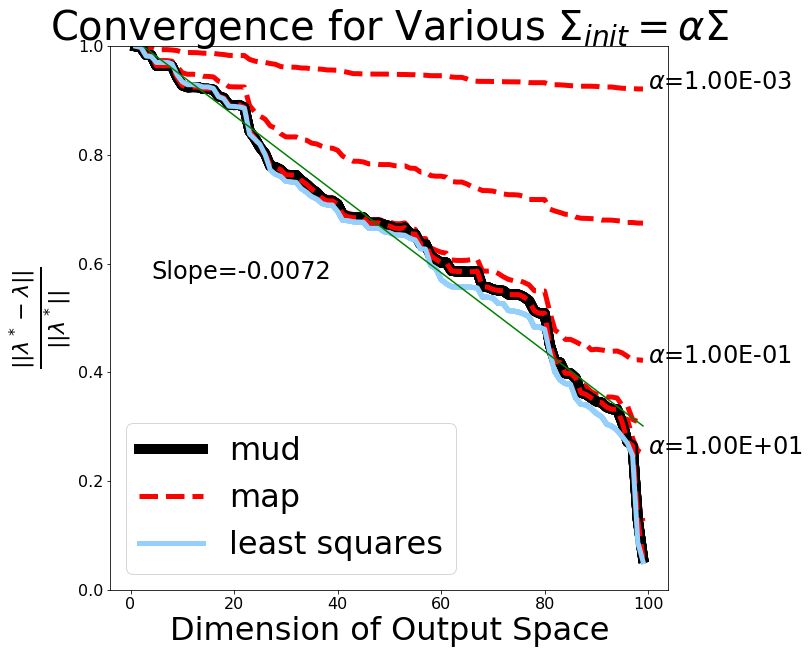
\includegraphics[width=0.475\linewidth]{figures/lin/lin-dim-cov-convergence}
  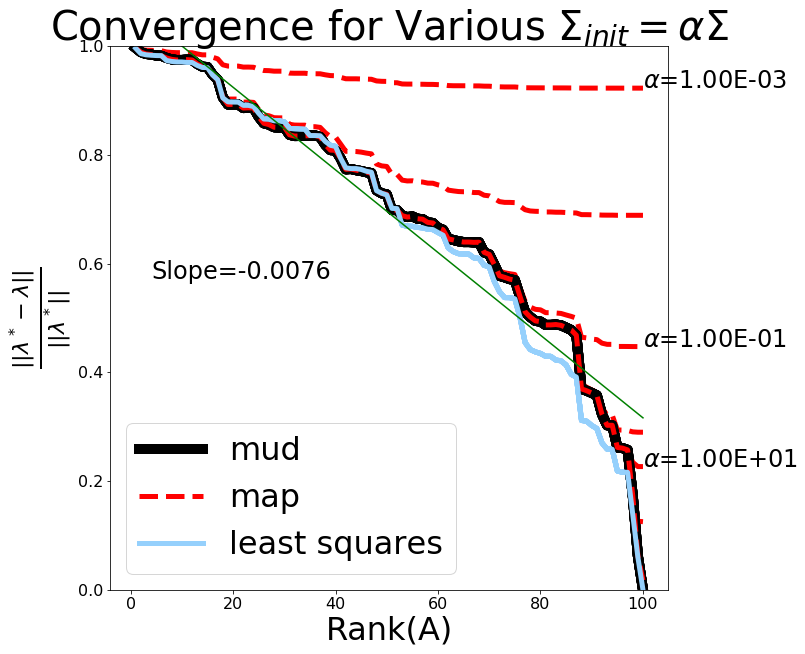
\includegraphics[width=0.475\linewidth]{figures/lin/lin-rank-cov-convergence}
\caption{
  Non-identity covariance
  (Left): Error for increasing dimensions of $D$ for $A$ taken to be a Gaussian Random Map (there's a name for these...).
  (Right): Error for increasing row-rank of $A$.
  (Bottom): Corresponding residuals between the least squares solution obtained through `numpy`'s `linalg.pinv` module and the closed-form solution for the MUD point given in Eq~\eqref{eq:mud-point-analytical-final}.
}
\label{fig:lin-error}
\end{figure}


\subsection{Impact of Output Dimension}%: Random $\RR^{k\times 100}$ matrix for $k=1,2,\ldots,100$}


%Here, we demonstrate how the various estimates of a true parameter $\paramref$ are impacted by the number of available QoI.%, especially in problems where the dimension of $\pspace$ is high.
%As more QoI are incorporated, the expectation is that the accuracy of $\paramref$ improves as well.
%In the following example, we demonstrate that the MUD point does indeed perform this way, and compare its ability to approximate $\paramref$ against two other popular solution methods: the least-squares solution and Tikhonov-regularized solution, i.e. the MAP point.

We consider QoI defined by $A\param+\mathbf{b}$ for $A\in\RR^{k\times 100}$ where $k=1,2,\ldots,100$ to demonstrate how the various estimates of a true parameter $\paramref$ are impacted by the number of available QoI.
To generate the matrices, we first generate $10,000$ independent identically distributed (i.i.d.) random numbers from a $N(0,1)$ distribution that are arranged into a reference $\RR^{100\times 100}$ matrix.

The same distribution is also used for generating the components of the 100-dimensional vectors defining a reference bias vector $\mathbf{b}$ and reference parameter $\paramref$.
A multivariate Gaussian distribution is used for the initial density, with zero mean and $\initialCov$ chosen as a diagonal covariance with random entries drawn from $U[0.5, 1.5]$ and sorted in descending order.%\footnote{A random seed of $271$ is used so that the covariance in this example matches that in the following, where we perform a similar study but vary the row-rank of $A$ instead of the dimension.}
%We then attempt to recover $\paramref$ with the three solution methods: MUD, MAP, and Least Squares, leveraging analytical solutions for all three since we have posed a linear problem under Gaussian assumptions.
The prior density is also a zero mean multivariate Gaussian distribution.
However, to demonstrate the impact of the strength of prior beliefs on the MAP point, we choose the prior covariance to be $\alpha\initialCov$  for $\alpha=0.001, 0.01, 0.1, $ and $10$.
Here, smaller values of $\alpha$ correspond to a ``stronger'' belief in the prior since the prior density becomes more concentrated near the prior mean.


To study the impact of dimension on the MUD, MAP, and least squares estimates, we solve a
sequence of inverse problems by truncating the rows of the reference matrix and bias vector.
%
%We scale the initial covariance $\initialCov$ by a factor $\alpha$ for $\alpha = 0.01, 0.1, 1, 10 $ to simulate varying levels of attachment to the specification of the initial density.
The results are summarized in the left plot of Figure~\ref{fig:lin-error}, which shows convergence towards $\paramref$ for all the problems considered with the exception of several MAP estimates corresponding to strongly-held beliefs in the prior.


%We demonstrate that the MUD solution retains the accuracy of least squares solutions while simultaneously offering the flexibility of specifying initial beliefs.
%Normally in order to incorporate such beliefs, one would perform Tikhonov regularization, usually with the inclusion of a hyper-parameter which scales the additional parameter-space norm in the objective function.
%Mathematically, this scaling factor applied to the norm is equivalent to scaling the matrix representation of the initial (prior) covariance.
%Increasing this scaling factor is interpreted as having less confidence in these initial assumptions.
%Conversely, decreasing it is equivalent to putting more emphasis on the prior beliefs than the evidence provided by the data, which causes MAP solutions to drift away from the solution contour (equivalence class) to which $\paramref$ belongs.
%The MUD point, by contrast, is not impacted by such a scaling of the initial covariance, providing \emph{consistent} solutions which demonstrate levels of accuracy that MAP points only exhibit for larger values of scaling factors.

%To illustrate this with a concrete example, we consider the problem $A\param + b = y$ by first generating a square matrix $A$ of dimension $100$ with standard Gaussian entries.
%The same distribution is used for the components of vector $b$ and $\paramref$ as well.
%A Gaussian distribution is used for the initial density, with mean at the origin (to complement the structure imposed by the least-squares framework), and a diagonal covariance with entries drawn from $U[0.5, 1.5]$ and sorted in descending order.\footnote{A random seed of $271$ is used so that the covariance in this example matches that in the following, where we perform a similar study but vary the row-rank of $A$ instead of the dimension.}
%We then attempt to recover $\paramref$ with the three solution methods: MUD, MAP, and Least Squares, leveraging analytical solutions for all three since we have posed a linear problem under Gaussian assumptions.
%To study the impact of dimension, we solve inverse problems for a sequence of maps generated by truncating the rows of $A$.
%Finally, several scalings of the initial covariance are chosen to simulate a common procedure in the Bayesian literature: hyper-parameter optimization.
%We scale the initial covariance $\initialCov$ by a factor $\alpha$ for $\alpha = 0.01, 0.1, 1, 10 $ to simulate varying levels of attachment to the specification of the initial density.
%The results are summarized in Figure~\ref{fig:lin-error}, which shows convergence towards $\paramref$ for all the problems considered with the exception of several Tikhonov solutions corresponding to strongly-held beliefs in initial assumptions about parameters.

We note that the MUD solution is the same for all choices of $\alpha$ and corresponds to the same level of accuracy that the MAP point achieves when $\alpha$ is chosen to be large.
In other words, the MUD point is not impacted by a scaling of the initial covariance, providing \emph{consistent} solutions which demonstrate levels of accuracy that MAP points only exhibit for larger values of scaling factors.
%The accuracy of the Tikhonov solution is highly dependent on the specification of $\initialCov$ and in some cases leads to nearly-divergent scenarios.

Of interest is also that the MUD point can sometimes out-perform the least squares estimate while generally achieving similar levels of accuracy.
This suggests that the MUD point has several favorable qualities.
Not only is it robust to the specification of prior assumptions, but it manages to offer the flexibility of incorporating good prior specifications without paying the additional cost of hyper-parameter optimization (i.e., choosing an appropriate $\alpha$) that would be required for the MAP estimates to achieve comparable results.

While omitted in the interest of space, if $\initialCov$ is chosen as $\alpha I$, where $I$ denotes the identity matrix of appropriate dimensions, then the MUD point will always agree with the least squares estimate.
Taking these results together, this implies that only a good ``relative spatial structure'' of prior beliefs is required to improve the MUD point's accuracy over both MAP and least squares estimates.


\subsection{Impact of Rank: One Hundred (Deficient) $\RR^{100 \times 100}$ matrices}

Here, we investigate whether the previous dimension-dependent example extend to matrices $A$ which are of a fixed dimension but varying rank.
This is of interest in applications where many QoI are available to construct an operator but a great deal of redundancy may be present in the data collected, and feature-engineering new quantities is somehow prohibitive (perhaps due to gradient estimation).

%The theory implies that a full-rank operator $A$ whose input and output dimensions are equal would ``turn off'' the data-consistent regularization, since the predicted covariance $\predictedCov = A^T \initialCov A$ is invertible.

The rank of $A$ corresponds to the number of unique directions of information present in the operator, i.e., how many directions in the parameter space are informed by the QoI map.
%, in other words, the mutual-distinctness of the information in the Quantities of Interest.
The operators in the previous example were all full rank, so the dimension of each map also corresponded to the rank of $A$.
When $A$ is rank-deficient, $\predictedCov$ is non-invertible, so we must modify the form of \eqref{eq:mud-point-analytical-final} to substitute a pseudo-inverse for the predicted covariance.
% we are curious to see if the same behaviors are observed on this related problem which violates one of the stated assumptions in the theory presented in section [TK - section with theory in it].


In this example, the dimension of the data space remains fixed at $d=100$ across all experiments.
However, we sequentially increase the row-rank of $A$ from $r=1, \ldots, 100$.
To control the rank of $A$, we first construct a reference $\RR^{100\times 100}$ matrix as in the previous example using 10,000 i.i.d. $N(0,1)$ random numbers.
We then compute a singular value decomposition of this reference matrix of the form $USV^\top$ and construct 100 rank-1 matrices of the form $A_i=\mathbf{u}_i s_i \mathbf{v}_i^\top$ for $i=1,\ldots,100$ where $\mathbf{u}_i$ and $\mathbf{v}_i$ denote the $i$th columns of $U$ and $V$, respectively and $s_i$ denotes the $i$th singular value.
Then, we analyze the impact of $A = \sum_i^r A_i$ for $r=1,\ldots,100$.
%\footnote{We validated by alternatively generating rank-1 matrices from random Gaussian vectors $a_i \in \RR^100$ to form $A_i = a_i a_i^T$, and included assertion checks in code to validate correct rank with our generating functions.}.
Aside from the differing construction of $A$, the rest of the choices involved in the experiment ($\paramref$, the reference bias vector, and the distributions involved) is identical to the previous example.

In the right plot of Figure~\ref{fig:lin-error}, we
%super-impose the pseudo-inverse solution in light blue and see that it matches the black line associated with the MUD error much of the time.
again find that the MUD point is generally as accurate as the least squares estimate, but incorporates an initial description of uncertainty, which may allow it to outperform the least squares estimate.
Also, we again see that the MAP estimates are impacted by the strength of prior beliefs.



%%%%%%%%%%%%%%%%%%%%%%%%%%%%%%%%%%%%%%%%%%%%%%%%%%%%%%%%%%%%%%%%%%%%
%%%%%%%%%%%%%%%%%%%%%%%%%%%%%%%%%%%%%%%%%%%%%%%%%%%%%%%%%%%%%%%%%%%%
\section{Data-constructed QoI maps and MUD points}\label{sec:data-maps}

Suppose there exists $d$ measurement devices for which repeated noisy data are obtained.
For each $1\leq j\leq N$, denote by $\mathcal{M}_j(\paramref)$ the $j$th measurement device, and denote by $N_j$ the number of noisy data obtained for $\mathcal{M}_j(\paramref)$.
Let $d_{j,i}$ denote the $i$th noisy datum obtained for the $j$th measurement where $1\leq i\leq N_j$.
To simplify the presentation and some of the resulting notation, we assume an unbiased additive error model for the measurement noise with independent identically distributed (i.i.d.) Gaussian errors so that
\begin{equation}\label{eq:obs_data_error}
	d_{j,i} = M_j(\param^\star) + \xi_i, \ \xi_i\sim N(0,\sigma_j^2), \ \ 1\leq i\leq N_j.
\end{equation}

%%%%%%%%%%%%%%%%%%%%%%%%%%%%%%%%%%%%%%%%%%%%%%%%%%%%%%%%%%%%%%%%%%%%
%%%%%%%%%%%%%%%%%%%%%%%%%%%%%%%%%%%%%%%%%%%%%%%%%%%%%%%%%%%%%%%%%%%%
\subsection{The Weighted Mean Error Map}

We now construct a $d$-dimensional vector-valued map from data obtained on the $d$ measurement devices.
The data-defined QoI map we consider in this work is referred to as the weighted mean error (WME) map, denoted by $Q_\text{WME}(\param)$ with $j$th component, denoted by $Q_{\text{WME},j}(\param)$, given by
\begin{equation}\label{eq:qoi_WME}
	Q_{\text{WME},j}(\param) := \frac{1}{\sqrt{N_j}} \sum_{i=1}^{N_j} \frac{M_j(\param)-d_{j,i}}{\sigma_j}.
\end{equation}
%%\begin{equation}\label{eq:qoi_WME}
%%	Q_{(\param,\xi) := \frac{1}{\sqrt{S}} \sum_{j=1}^S \frac{M_j(\param)-d_j(\xi_j)}{\sigma_j}.
%%\end{equation}
By a substitution of \eqref{eq:obs_data_error} into \eqref{eq:qoi_WME} and rationalizing the denominator of the multiplicative factor, $Q_{\text{WME},j}(\paramref)$ is identified as the sample average of $N_j$ random draws from an i.i.d.~$N(0,N_j)$ distribution.
By assumption, the observed data are generated according to the fixed true physical parameter vector given by $\paramref$ in \eqref{eq:obs_data_error}.
Subsequently, each component of $Q_\text{WME}(\paramref)$ is a random draw from an $N(0,1)$ distribution.
Therefore, with this choice of data-defined QoI map, we specify $\observed$ as a $N(\mathbf{0}_{d\times 1},\mathbf{I}_{d\times d})$ distribution.


%%%%%%%%%%%%%%%%%%%%%%%%%%%%%%%%%%%%%%%%%%%%%%%%%%%%%%%%%%%%%%%%%%%%
%%%%%%%%%%%%%%%%%%%%%%%%%%%%%%%%%%%%%%%%%%%%%%%%%%%%%%%%%%%%%%%%%%%%
\subsection{Analysis of MUD point for the WME map}\label{sec:MUD_analysis}
%%%%%%%%%%%%%%%%%%%%%%%%%%%%%%%%%%%%%%%%%%%%%%%%%%%%%%%%%%%%%%%%%%%%
%%%%%%%%%%%%%%%%%%%%%%%%%%%%%%%%%%%%%%%%%%%%%%%%%%%%%%%%%%%%%%%%%%%%

Below, we consider issues of existence, uniqueness, and convergence of $\mudpt$ for the WME map under certain assumptions.
In~\ref{sec:Conclusions}, we provide some remarks on how we plan to generalize this analysis in future work.


For each $1\leq j\leq M$, assume that the observable maps $M_j$ are linear maps of $\param$ (affine maps require minor modifications to the results below).
For notational simplicity below, assume that $M_j$ is written explicitly as a $1\times p$ row vector and that the $d$-vectors form a linearly independent set.
Then, it is possible to rewrite $Q_{\text{WME}}(\param)$ as
\begin{equation}
	Q_\text{WME}(\param) = A(\mathbf{N})\param + b(\mathbf{N}),
\end{equation}
where the $j$th component of $\mathbf{N}\in\RR^d$ is given by $N_j$ and the $j$th row of $A(\mathbf{N})\in\RR^{d\times p}$ is given by
\begin{equation}
	\frac{1}{\sqrt{N_j}} \sum_{i=1}^{N_j} \frac{M_j}{\sigma_j} = \frac{\sqrt{N_j}}{\sigma_j}M_j,
\end{equation}
and the bias vector, $\mathbf{b}(\mathbf{N})\in\RR^d$, is defined by the data, with $j$th component, denoted by $\mathbf{b}_j$, given by
\begin{equation}
	\mathbf{b}_j(\mathbf{N}) = -\frac{1}{\sqrt{N_j}} \sum_{i=1}^{N_j} \frac{d_{j,i}}{\sigma_j}.
\end{equation}
Since $A(\mathbf{N})\initialCov A(\mathbf{N})^\top$ defines a predicted covariance, and the observed covariance is the identity map, the predictability assumption is immediately satisfied if each diagonal component of the predicted covariance is significantly greater than $1$.

The off-diagonal components of the predicted covariance (which are dictated in large part by the structure of the measurement operators $M_j$) dictate how much larger than $1$ each diagonal component must be to ensure the predictability assumption holds.
However, we demonstrate below that this will happen once a minimum number of data points $N_\text{min}$ are obtained for each measurement.

First, observe that the $j$th diagonal component of the predicted covariance matrix is  given by the predicted variance associated with using the scalar-valued map $Q_{\text{WME},j}$.
Then, the associated predicted variance is given by
\begin{equation}
	\frac{N_j}{\sigma_j^2} M_j\initialCov M_j^\top
\end{equation}
Since $\initialCov$ is assumed to be non-degenerative and $M_j$ is a non-trivial row vector, this predicted variance grows linearly with $N_j$.
In other words, the $j$th diagonal component of the predicted covariance has the form $\beta_j N_j$ for some $\beta_j>0$.
Let $N_{\text{min},j}$ denote the minimum $N_j$ for $1\leq j\leq N$ necessary to make the $j$th diagonal components sufficiently large so that the smallest eigenvalue of the predicted covariance is larger than $1$ (which is the repeated eigenvalue for the observed covariance).

The following result is now an immediate consequence of Theorem~\ref{thm:MUD_existence_uniqueness},

\begin{corollary}\label{cor:MUD_wme}
If $\initial \sim N(\param_0,\initialCov)$ and data are obtained for $d$ linearly independent measurements on $\pspace$ with an additive noise model with i.i.d. Gaussian noise for each measurement, then there exists a minimum number of data points obtained for each of the measurements such that there exists a unique $\mudpt$ and $Q_\text{WME}(\mudpt) = 0$.
\end{corollary}



%%%%%%%%%%%%%%%%%%%%%%%%%%%%%%%%%%%%%%%%%%%%%%%%%%%%%%%%%%%%%%%%%%%%
%%%%%%%%%%%%%%%%%%%%%%%%%%%%%%%%%%%%%%%%%%%%%%%%%%%%%%%%%%%%%%%%%%%%
\section{MUD points for nonlinear maps: Examples}\label{sec:Parameter-identification}
%%%%%%%%%%%%%%%%%%%%%%%%%%%%%%%%%%%%%%%%%%%%%%%%%%%%%%%%%%%%%%%%%%%%
%%%%%%%%%%%%%%%%%%%%%%%%%%%%%%%%%%%%%%%%%%%%%%%%%%%%%%%%%%%%%%%%%%%%

We now use MUD points as parameter estimates for nonlinear data-constructed maps using simulated noisy temporal and spatial data associated with solutions to differential equations.
The previously derived closed form expressions for $\mudpt$ do not apply in these examples.
Instead, in each example we use a fixed set of i.i.d.~samples drawn from the initial density to approximate the updated density and subsequently choose the sample that maximizes this approximation.
Future work will consider how to leverage more sophisticated optimization approaches for estimating $\mudpt$, e.g., through iterative quasi-Newton approaches based on repeated approximate linearizations that can exploit the closed form expressions for $\mudpt$.
%that are iteratively improved upon, e.g., by combining this work with a quasi-Newton type approach.

The two examples below have distinct points of emphasis.
The first example focuses on the improved accuracy and precision of scalar $\mudpt$ estimates as more data are incorporated into the construction of $Q_\text{WME}$.
The second example focuses on how the utilization of subsets of the data into different components of a vector-valued $Q_\text{WME}$ can improve the estimates across multiple components of a $\mudpt$ estimate for a parameter vector.
Despite these differences, both examples share the following details.
\begin{itemize}
  \item Sets of i.i.d.~samples from the initial densities are used to both approximate the predicted density (and thus the updated density) and to form a discrete space in which to search for the MUD point.
  \item A reference parameter is chosen and used to establish a (noiseless) reference solution (in space or time).
  \item An i.i.d. additive noise model with $\xi \sim N(0,\sigma^2)$ is used to perturb the reference temporal and spatial solutions.
  \item Since the magnitude of solutions in both examples is $\mathcal{O}(1)$, noise variances are chosen so that $\mathbb{P}( \abs{\xi} < \tau ) = 99\%$, with $\tau=0.1$. In other words, we simulate an ``engineering accuracy'' by permitting measurement noise to vary by  approximately 10\% of the signal magnitude.
%  \item Vertical axes on convergence plots represent the absolute error between $\paramref$ and $\mudpt$, with bounds chosen to be fixed across plots within a figure.
%  \item Errors are reported as the average over 20 sets of independently generated noisy data.
%  \item To estimate convergence rates, we compute first-order linear regressions for the logarithm (base 10) of the mean and variances for the absolute error. The coefficient for the mean in the regression appears as an annotation in the figures.
\end{itemize}

%%%%%%%%%%%%%%%%%%%%%%%%%%%%%%%%%%%%%%%%%%%%%%%%%%%%%%%%%%%%%%%%%%%%
\FloatBarrier
%%%%%%%%%%%%%%%%%%%%%%%%%%%%%%%%%%%%%%%%%%%%%%%%%%%%%%%%%%%%%%%%%%%%

\subsection{ODE Example}\label{subsec:ode-example}
\begin{figure}[htb]
  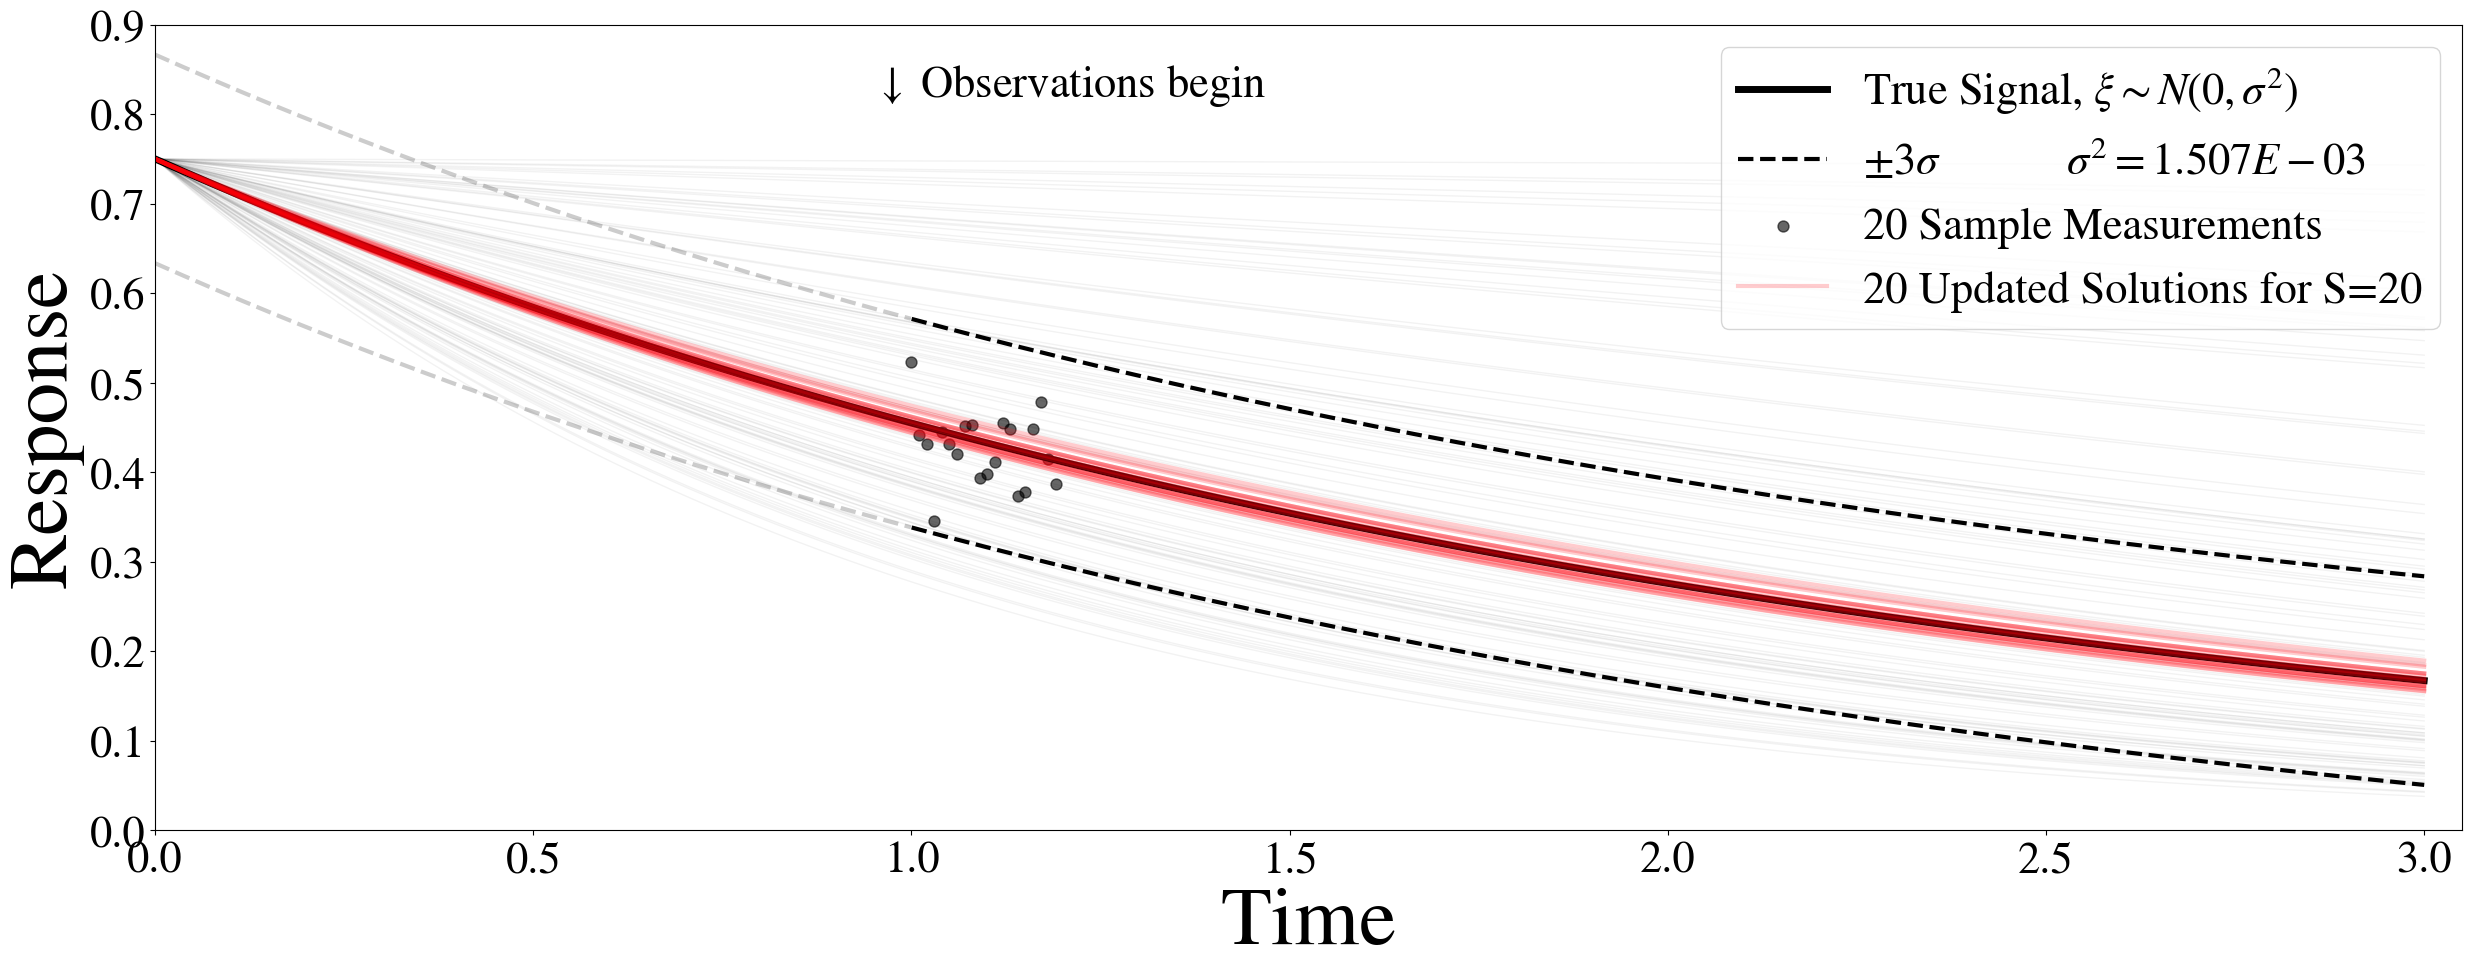
\includegraphics[width=\linewidth]{figures/ode/ode_20_reference_solution}
  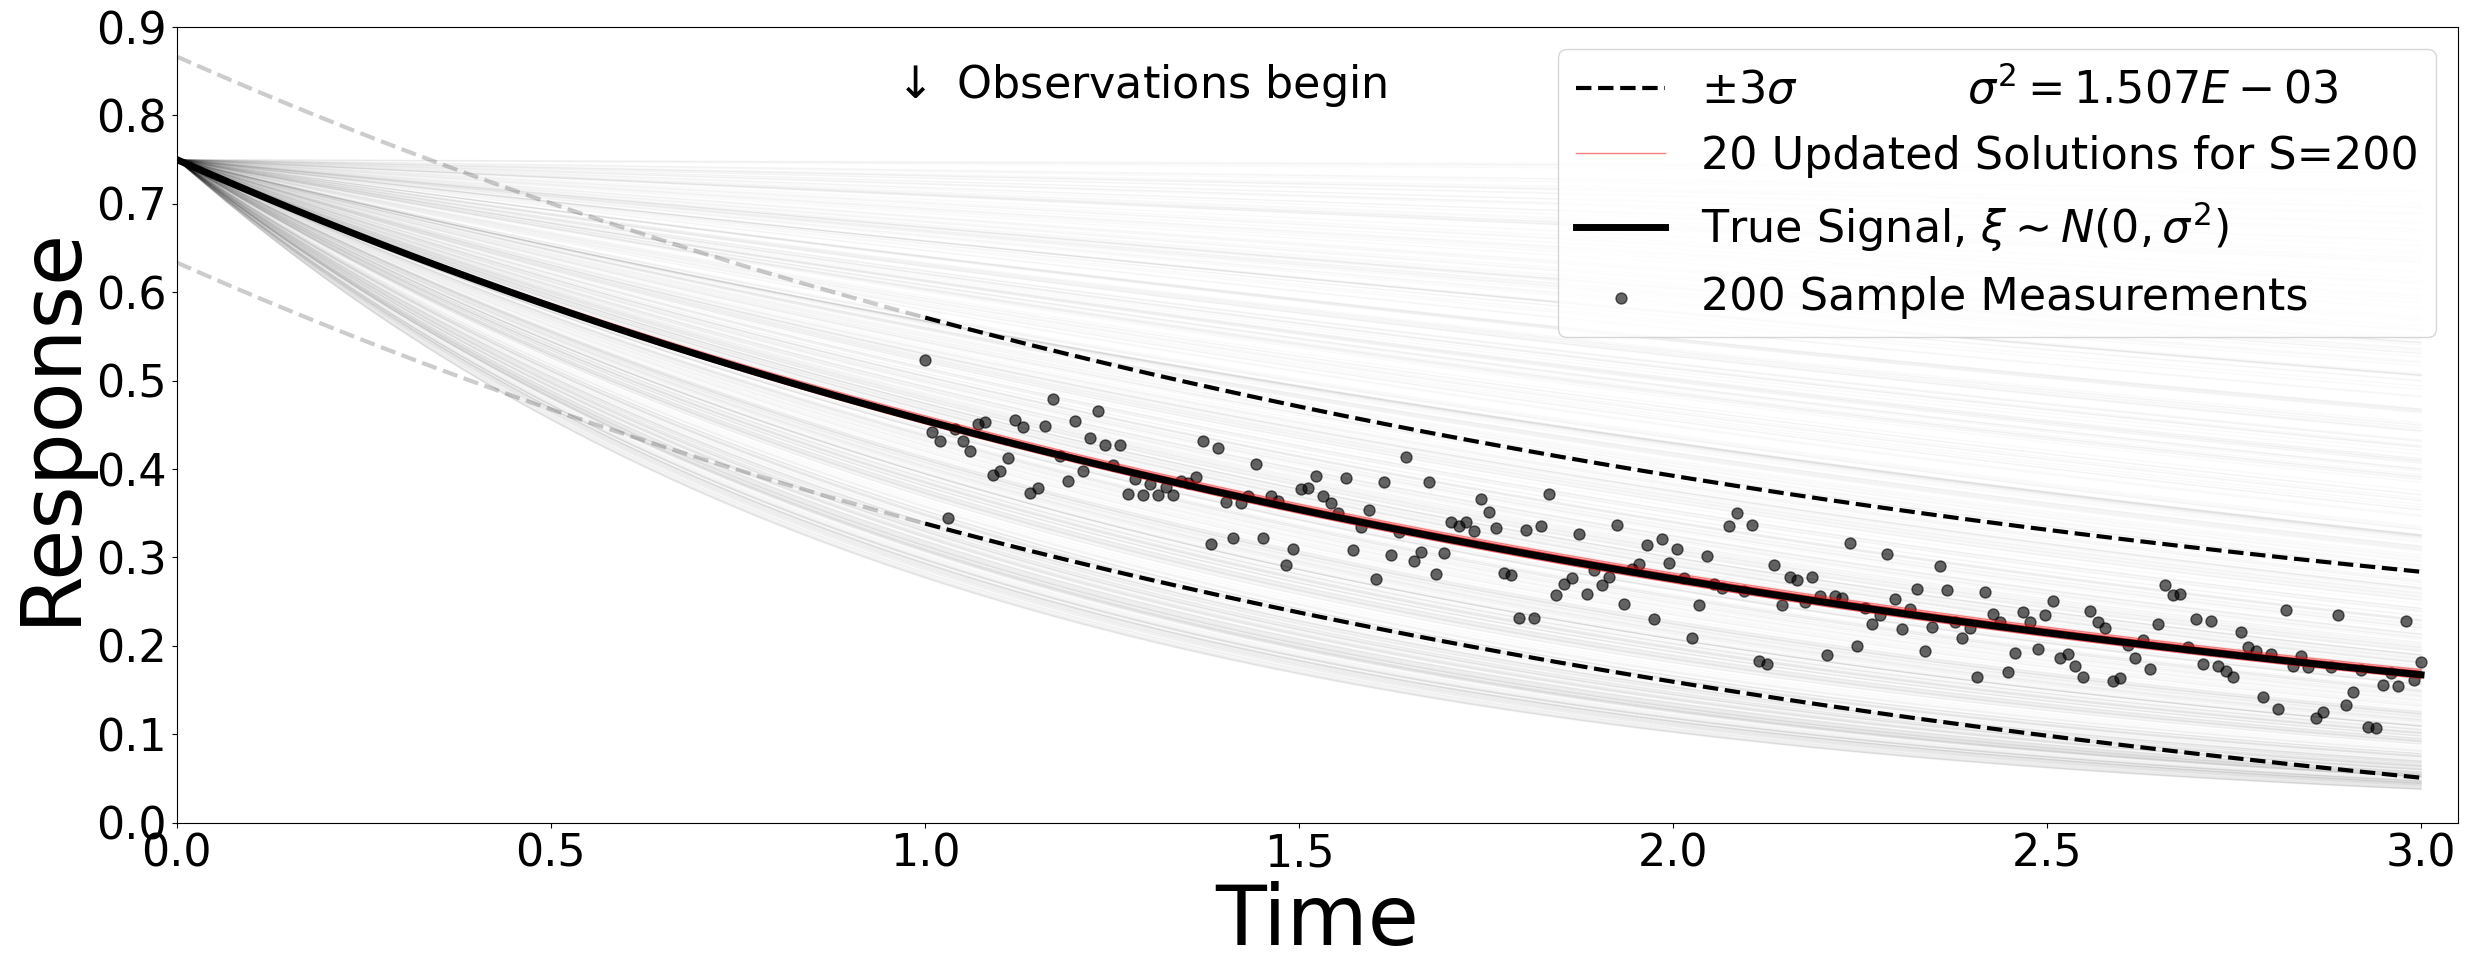
\includegraphics[width=\linewidth]{figures/ode/ode_200_reference_solution}
  \caption{Curves for exponential decay model with various decay coefficients. Dashed curves denote 99\% probability intervals for noise. The true signal is shown in solid black.
 Curves associated with the MUD estimates for the decay coefficient computed from 20 trials are shown in light red.
 Both sets of these curves encompass the true signal for $N=20$ (top plot) and $N=200$ (bottom plot) data points.
 The light red curves are almost indistinguishable in the bottom plot as they all lie nearly on the true signal which demonstrates the overall reduction in variance in MUD estimates around the true signal when using $N=200$ data points.
	{
	\color{blue}{First line of legend: ``$\pm 3\sigma$ from True Signal''. Second line of legend: ``True signal''. Third line ``Measurements with $N(0,\sigma^2)$ noise''. Then, fourth line of legend: ``Signals based on $\mudpt$ estimates''. Also, make the red curves dash-dotted and less transparent so that they are easier to distinguish. Maybe use a deeper red. }
	}
  }
  \label{fig:ode-reference}
\end{figure}

\begin{figure}[htb]
  \centering
  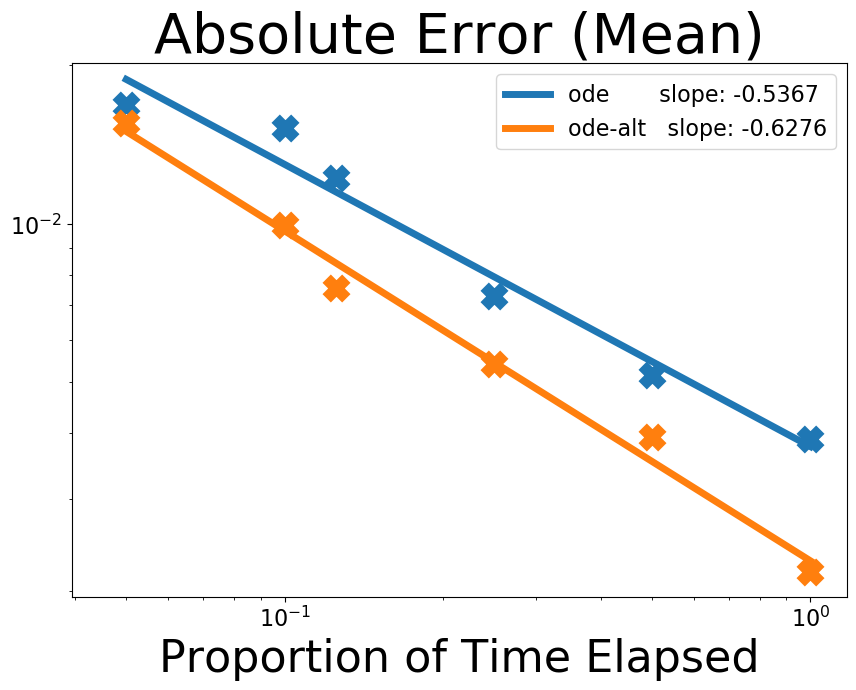
\includegraphics[width=0.4\linewidth]{figures/ode/ode_convergence_mud_obs_mean}
  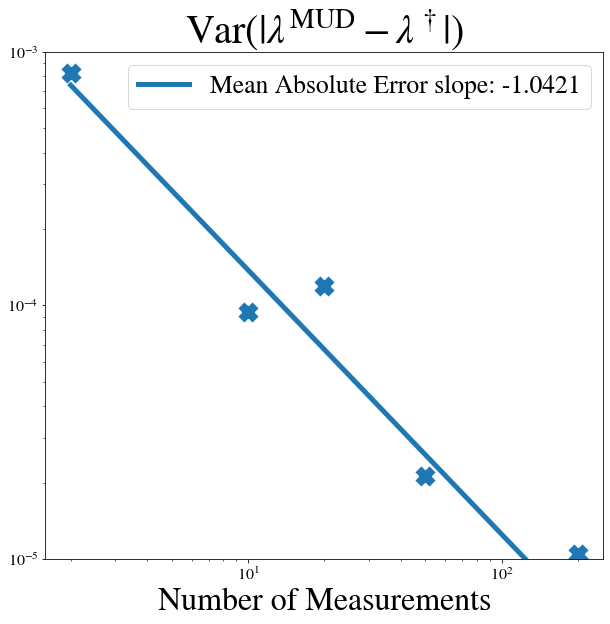
\includegraphics[width=0.4\linewidth]{figures/ode/ode_convergence_mud_obs_var}
  \caption{The mean (left) and variance (right) of absolute errors in MUD estimates as a function of the number of data points used. These statistics are computed over 20 trials.
  {
  \color{blue}{Change "Proportion of Time Elapsed" to "N" and plot vs $N$. Remove the orange scatter points and curves. Change titles to $\mathbb{E}(\abs{\mudpt - \paramref})$ and $Var(\abs{\mudpt-\paramref})$.}
  }
  }
  \label{fig:ode-convergence-obs}
\end{figure}

Consider the exponential decay problem with uncertain decay rate $\param$:
$$
\begin{cases}
\frac{\partial u}{\partial t} & = \param u(t), \ 0<t\leq 3, \\ u(0) &= 0.75,
\end{cases}
$$
with solution
\begin{equation}
  u(t;\param) = u_0\exp(-\param t), \; u_0 = 0.75 ,
\end{equation}
and measurements begin at $t=1$.

The initial uncertainty in the decay rate is given by a uniform density on $\param \in \Lambda = (0, 1)$, and $10,000$ samples from this density are used to estimate the push-forward and updated densities as well as the MUD points.
Noisy data are simulated over the interval $t \in [1,3]$ assuming a $100$Hz measurement sensor.
An example of this setup is shown in Figure~\ref{fig:ode-reference}, with the solid line representing the ``true'' signal obtained by evaluating the solution for $\paramref = 0.5$, and a particular realization of noisy data shown as perturbed points around it.

For 20 different realizations of $N=5, 10, 15, 20, 25, 50, 100, \text{ and } 200$ noisy measurement data, we construct $Q_\text{WME}$ with $u(t;\param)$ replacing $M_j(\param)$ in~\eqref{eq:qoi_WME}, estimate $\mudpt$, and analyze the statistical error in these estimates of $\paramref$.
In the left plot of Figure~\ref{fig:ode-convergence-obs}, we observe that as more data are used that the accuracy (defined by the mean error between $\mudpt$ and $\paramref$) decreases.
The right plot demonstrates that the precision (i.e., the variance in the error) is also reduced by using more data.
These results are also visualized in the plots of Figure~\ref{fig:ode-reference} where the distinct red curves in the top plot are the signals associated with the 20 $\mudpt$ estimates associated with the 20 independent trials of $N=20$ noisy measurements.
However, in the bottom plot, these 20 red curves are fairly indistinguishable to the naked eye from the true signal when using $N=200$ noisy measurements.


%%%%%%%%%%%%%%%%%%%%%%%%%%%%%%%%%%%%%%%%%%%%%%%%%%%%%%%%%%%%%%%%%%%%
\FloatBarrier
%%%%%%%%%%%%%%%%%%%%%%%%%%%%%%%%%%%%%%%%%%%%%%%%%%%%%%%%%%%%%%%%%%%%

\subsection{PDE Example}\label{subsec:pde-example}

In this problem, the uncertain model parameter is now described by an unknown function defining the boundary data to a stationary PDE.
The focus is on demonstrating that a vector-valued QoI can be constructed from noisy data to produce a MUD point that more accurately reconstructs features of the unknown function.
As described below, there is an intuitive way to separate the spatial data to construct the distinct components of the vector-valued QoI map.
While beyond the scope of this work, a future work will consider how to incorporate clustering analysis on the data for less obvious cases where we seek to determine which data points should be utilized to construct the various components of a vector-valued QoI map.
In the interest of space and clarity, we present representative results for a fixed finite-dimensional representation of the parameter space and forgo the more complicated convergence analysis that requires increasing both the number of data available as well as the dimension of the parameter space.

Consider the Poisson problem:
\begin{equation}\label{eq:pde-equation}
\begin{cases}
\hfill -\nabla \cdot \nabla u &= f(x), \quad\text{on } x\in \Omega, \\
\hfill u &= 0, \quad\text{ on } \Gamma_T \cup \Gamma_B, \\
\hfill \frac{\partial u}{\partial \mathbf{n}} &= g(x_2), \quad\text{ on } \Gamma_L, \\
\hfill \frac{\partial u}{\partial \mathbf{n}} &= 0, \quad\text{ on } \Gamma_R,
\end{cases}
\end{equation}
where $x=(x_1, x_2) \in \Omega = (0,1)^2$ is the spatial domain; $\Gamma_T$, $\Gamma_B$, $\Gamma_L$, and $\Gamma_R$, denote the top, bottom, left, and right boundaries of this domain, respectively, and $\frac{\partial u}{\partial \mathbf{n}}$ denotes the usual outward normal derivative.
The forcing function $f$ is taken to be $10\exp{\norm{x - 0.5}^2 / 0.02}$.

Here, we assume that $g(x_2)$ is unknown, and the goal is to use noisy data to estimate this unknown boundary data.
In other words, the parameter $\param$ now represents an uncertain function.
To generate the noisy data, we first use a reference $g(x_2)\propto x_2^2(x_2-1)^5$ with a constant of proportionality chosen to produce a minimum of $-3$ at $x_2=\frac{2}{7}$.
Then, we compute a reference solution using piecewise-linear finite elements on a triangulation of a $36x36$ mesh.
Random noise is then added to every degree of freedom of this reference solution, and the spatial data are subsequently computed from a fixed set of 100 randomly placed sensors in the subdomain $(0.05, 0.95)^2 \subset \Omega$.
This process is repeated $20$ times to study the subsequent variation in MUD points due to different realizations of noisy data.
See the plot of Figure~\ref{fig:pde-Q} for a representative noisy response surface and location of spatial data used across all 20 trials.

\begin{figure}[htbp]
\centering
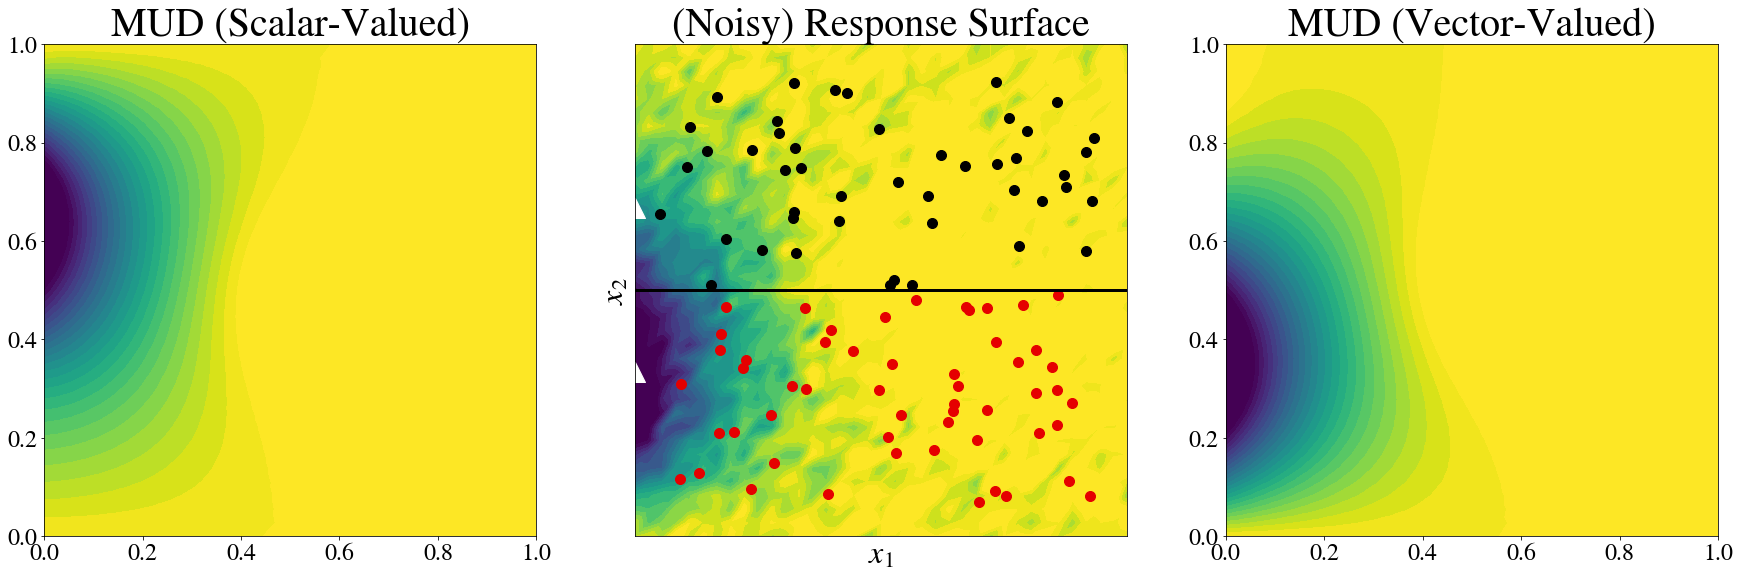
\includegraphics[width=0.95\linewidth]{figures/pde-highd/pde-highd_surf_exmud_D2_m100}
\caption{
{\color{blue}Just use center plot.}
A representative noisy perturbation of the reference response surface. Locations of the randomly chosen spatial data used to construct both $Q_{1D}$ and $Q_{2D}$ are shown as black and red dots.
}
\label{fig:pde-Q}
\end{figure}

%We simulate measurement noise as described in the preamble to Sec.~\ref{sec:Parameter-identification} and use this data to construct a QoI map with which we solve a parameter identification problem which characterizes $g$.
To construct a finite-dimensional parameter space describing the initial uncertainty of $g(x_2)$, we first assume that it is known that $g$ is non-positive and bounded below by $-4$.
We further assume that $g$ is smooth enough to be reasonably approximated by a piecewise-linear continuous spline with four knots and that $g(0)=g(1)=0$.
Thus, the uncertainty is described by the values of the splines at the two interior knot points chosen as the equispaced points $1/3$ and $2/3$.
This defines a finite-dimensional parameter space described by $\pspace = [0,-4]^2$.
We generate $1000$ samples from an initial uniform density on $\pspace$ to (1) generate random spline functions and compute the (noise-free) data from solutions associated with these splines; and (2) estimate the push-forward and updated densities along with the MUD estimate of $g(x_2)$.
The randomly generated splines are shown in the left plot of Figure~\ref{fig:pde-MUD} along with the reference $g$ and its interpolant on these spline knots.
These same $1000$ samples are used across all $20$ realizations of random noisy data.


\begin{figure}[htbp]
\centering
    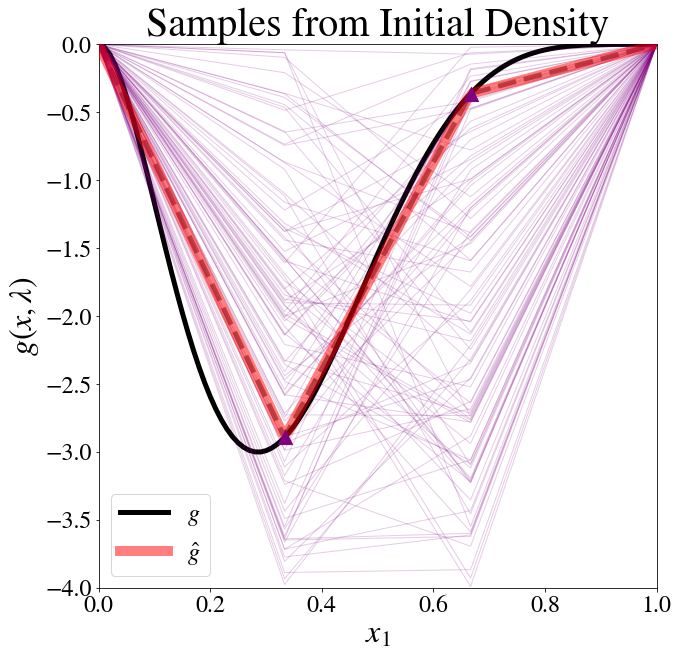
\includegraphics[width=0.325\linewidth]{figures/pde-highd/pde-highd_init_D2}
    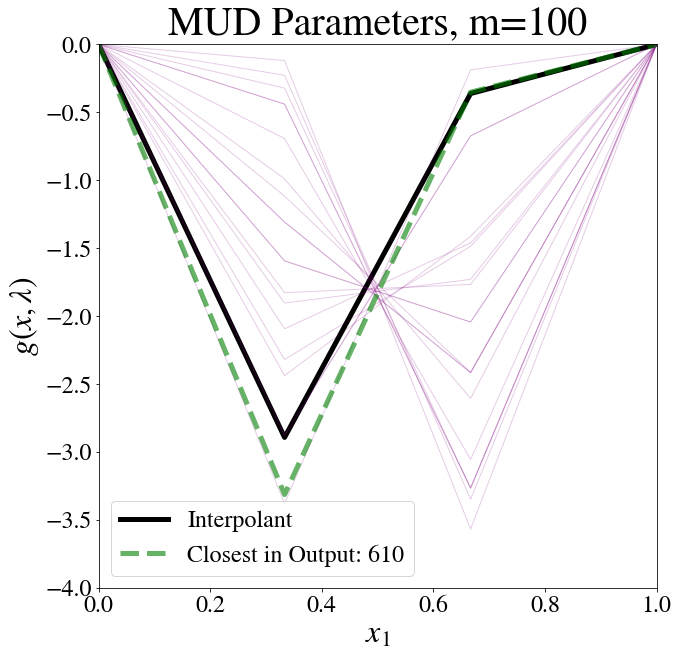
\includegraphics[width=0.325\linewidth]{figures/pde-highd/pde-highd_pair_D2-1_m100}
    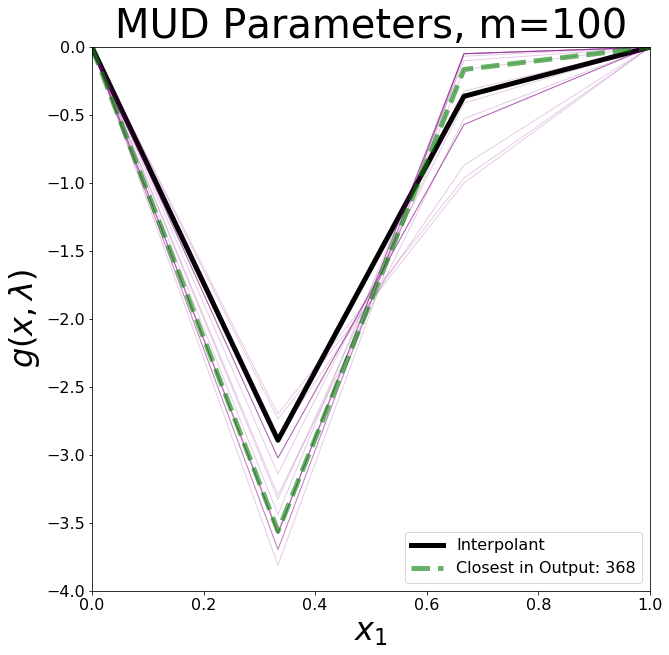
\includegraphics[width=0.325\linewidth]{figures/pde-highd/pde-highd_pair_D2-2_m100}
\caption{
{\color{blue}Remove the closest in output sample from all plots. Clean up legends and titles. Remove $m=100$. Titles for new center and right plots: ``MUD estimates for $Q_{1D}$'' and ``MUD estimates for $Q_{2D}$''. Legends for these plots: ``Interpolant of ref. $g$'' and ``MUD estimate of $g$''.
Title for new left plot: ``Initial estimates of $g$''. Legend: ``Reference $g$'' (the smooth curve), ``Interpolant of ref. $g$'' (piecewise-linear curve and use dashed curve for it), and ``Random initial est. of $g$'' (for the red curves).}
In the left plot, the reference $g(x_2)$ is shown as the solid black curve with its interpolant onto the spline basis shown as a dashed black curve.
The red curves {\color{blue}\bf Make more opaque} in the center and right plots show the variability in MUD estimates of $g(x_2)$ for the 20 different realizations of noisy data.
The center plot uses $Q_{1D}$ and the right plot uses $Q_{2D}$ to construct the MUD estimates.
}
\label{fig:pde-MUD}
\end{figure}


Two separate types of data-constructed $Q_\text{WME}$ maps are constructed from the data.
The first map, which for simplicity we denote by $Q_{1D}$, uses all 100 spatial data points to construct a scalar-valued QoI map.
Given the location of the spline knots, a second map, which for simplicity we denote by $Q_{2D}$, uses the data points above (below) the mid-line of the spatial domain to form the first (second) component of the 2-dimensional vector-valued QoI map.
This separation of spatial data is illustrated in the top-left plot in Figure~\ref{fig:pde-Q}.

%The top-center and top-right plots in Figure~\ref{fig:pde} illustrate solutions associated with the MUD estimates of $g(x_2)$ obtained from $Q_{1D}$ and $Q_{2D}$, respectively, using the noisy data shown in the top-left plot.

The center and right plots in Figure~\ref{fig:pde-MUD} shows the variability in the $20$ MUD estimates of $g(x_2)$ obtained from the different realizations of noisy data using $Q_{1D}$ and $Q_{2D}$, respectively.
For reference, the interpolant of the reference $g(x_2)$ on the spline basis is also shown in these plots.
Comparing these plots, we see that the MUD estimates associated with $Q_{2D}$ have less spatial variability than those associated with $Q_{1D}$ while also being better pointwise estimates for this interpolant of $g(x_2)$.
